\documentclass[lettersize,journal]{IEEEtran}

\usepackage{amsmath,amsfonts,amssymb}
\usepackage{array}
\usepackage{stfloats}
\usepackage{url}
\usepackage{graphicx}
\usepackage{cite}
\hyphenation{op-tical net-works semi-conduc-tor IEEE-Xplore}
\def\BibTeX{{\rm B\kern-.05em{\sc i\kern-.025em b}\kern-.08em
    T\kern-.1667em\lower.7ex\hbox{E}\kern-.125emX}}

\urlstyle{same}
\begin{document}

\title{Multirobot Tracking of Separatrices and
Objective Eulerian Coherent Structures}

\author{Christopher Waight and Christopher A. Kitts,~\IEEEmembership{Senior Member,~IEEE}
\thanks{C. Waight is a PhD Candidate in the Robotic Systems Laboratory, Department of Mechanical Engineering, Santa Clara University, Santa Clara, CA 95053 USA (e-mail: cwaight@scu.edu)}
\thanks{C. A. Kitts is Professor and Director of the Robotic Systems Laboratory, Department of Mechanical Engineering, Santa Clara University, Santa Clara, CA 95053 USA (e-mail: ckitts@scu.edu)}
}
\markboth{IEEE Systems Journal}%
{Waight and Kitts: Multirobot Tracking of Separatrices and Objective Eulerian Coherent Structures}

\maketitle

\begin{abstract}
Adaptive navigation is the process of modifying a robot's motion in
real time based on measurements taken while moving. This paper applies
that process to the boundaries that organize short-term transport in a
flow, the strain-dominated curves across which water masses separate
and along which floating material collects. Existing robotic trackers
of such structures either commit to the structure's identity before
tracking begins or accumulate an estimate over a finite integration
horizon. We present a six-robot cluster that does neither, locating
separating boundaries and holding station on attracting ones from the
instantaneous local flow measured simultaneously across the formation.
A cooperative estimator recovers the local quadratic field model from
one synchronous sample, six robots being the minimum for the
unconstrained model. That fit supplies two surrogates, the Jacobian
determinant, which traces separatrices but shifts under a rotating
observer, and the smaller rate-of-strain eigenvalue, which is objective
and recovers the identical material curve in any frame. We develop an
adaptive navigation primitive for each and characterize the tradeoff
between objectivity and noise tolerance. To our knowledge this is the
first demonstration of multirobot tracking of an objective Eulerian
coherent structure from instantaneous measurements alone. Monte Carlo
sweeps show the determinant tracker withstands about four to five times
more measurement noise, failing where the estimator gradient stops
being informative, while in a rotating-frame trial the strain tracker
holds the same material path and the determinant tracker departs the
structure. On Santa Barbara Channel radar currents both primitives
follow the same dominant transport corridor for nearly the full record,
separating only near landfall. The controllers are admittedly simple,
reactive, and minimal in robot count; even so, they demonstrate
acquisition, traversal, and terminal capture on both analytic and
measured fields, and yield an operational rule for selecting between
the two surrogates by observing platform and mission.
\end{abstract}

\begin{IEEEkeywords}
Multirobot Systems, Adaptive Navigation, Coherent Structures,
Okubo-Weiss, Rate of Strain, Objectivity, Cooperative
Estimation, Cluster Space Control
\end{IEEEkeywords}

\section{Introduction}

\IEEEPARstart{M}{ultirobot} systems offer redundancy, throughput, and
cooperative behaviors a single vehicle cannot produce, and they now
operate across land, sea, air, and space \cite{1}. Navigating an
unknown field is one such behavior. Rather than covering a region with
a prescribed survey trajectory, a cluster collects spatially
distributed readings at one instant, fits a local model of the
landscape around it, and steers on features of that model. This is
adaptive navigation (AN): the vehicle modifies its direction and path
in real time from measurements taken while moving \cite{2}. The sensing
argument favors the cluster. A single vehicle must translate to sense a
gradient, which costs time and misleads in a time-varying field,
whereas a cluster samples simultaneously, tolerates vehicle failures,
and adapts its size and shape to the spatial frequencies present
\cite{2,3}. Cluster size is a specifiable mission attribute, trading
spatial resolution, differential signal amplification, noise
suppression, and breadth of exploration against one another \cite{4}.

AN in scalar fields is well developed and supplies the pattern. Each
robot contributes one scalar measurement to a policy that reaches and
follows a feature, and formations are sized so that differential
measurements across the cluster recover the gradient and curvature the
policy consumes \cite{4,5}. \"{O}gren, Fiorelli, and Leonard
established cooperative gradient climbing with a formation of mobile
sensors \cite{5}; Bri\~{n}\'{o}n-Arranz, Renzaglia, and Schenato
extended it to the Hessian, five robots on a ring plus one at the
center recovering both in closed form \cite{4}; and McDonald, Kitts,
and Neumann developed and experimentally verified the ridge, trench,
and saddle primitives \cite{2,3,6}. A vector field carries its own
catalog of features. Critical points are the isolated members, sinks
and sources that mark convergence zones and subsurface leaks
\cite{7}, and in \cite{8} a three-robot cluster estimated the location
and type of one from a linear fit of simultaneous local velocity
measurements. Those
formations each sample a single signal channel; a coupled
two-component field doubles the estimation problem to twelve unknowns,
and \cite{4}'s fixed symmetric weights hold only for the ideal ring
geometry.

The extended features of a coastal flow are the subject here. Floating
material does not spread evenly, but collects along or separates across
the coherent structures of the flow: rotation-dominated cores that
retain whatever enters them, and strain-dominated boundaries across
which neighboring parcels are pulled apart. A separatrix is a transport
barrier, the curve a plume will not cross and the line along which a
coastal sensor array is best deployed \cite{9,10,11}; its saddle
points are the stagnation points where two barriers cross and the
corridor a drifter follows is decided. An attracting objective Eulerian
coherent structure (OECS) is an accumulator, the curve on which debris,
larvae, and search objects collect \cite{12}. Coordinated
multi-vehicle sampling of dynamic ocean features is an active area of
marine robotics \cite{13,14,15}. Knowing where these curves lie is the
difference between searching a corridor and searching a basin.

These structures are found today by one of two routes. Haller and Yuan
formalized the Lagrangian coherent structure (LCS) as the
generalization of stable and unstable manifolds to arbitrary time
dependence \cite{9}, computed as a ridge of the finite-time Lyapunov
exponent field \cite{11}; objectivity, the Lagrangian/Eulerian
tradeoff, sparse-trajectory gradient recovery, and the strain-spin
decomposition are adjacent active directions \cite{16,17,18,19,20}. The
instantaneous criteria are the computable alternative: Okubo and Weiss
partition a planar flow from the local velocity gradient alone
\cite{21,22}, generalized to three dimensions \cite{23}, refined for
oceanographic use \cite{24}, and applied at scale in mesoscale eddy
censuses \cite{25}. Both routes characterize the structure offline from
a reconstructed field, depend on an integration horizon that delays
all estimates, and assume the structure's identity before tracking
begins.

The nearest robotic work tracks a structure directly with a formation
and inherits that gap. Michini et al. bracket a presumed stable or
unstable manifold with three robots using only local velocity
measurements \cite{26}, extended to $N$ robots \cite{27} and validated
on micro surface vehicles \cite{28,29}. Its robots begin on the
manifold and are advected by the flow, the manifold's identity is
supplied in advance, and the saddle point is treated by neither the
controller nor its analysis; \cite{26} reports veering away from the
structure near a saddle in both flow-tank and ocean trials. Kularatne
and Hsieh instead compute the local FTLE field on board, recovering
type at the cost of a nonzero integration horizon \cite{30}.

This paper contributes a) a cooperative second-order estimator that
recovers the local quadratic model of a two-component field from one
synchronous sample, with six robots proved minimal, a conic
characterization of the formations that fail, and exact,
heading-isotropic noise gains, one per derivative order, that make
cluster size a specifiable mission attribute rather than a tuning
choice; b) two AN primitives, the $D$ tracker and the $s_1$ tracker,
that read the two terms of one splitting identity, $D = \omega^2/4 -
s_1^2$, off the same six-robot fit, demonstrating acquisition,
traversal, and terminal capture where the model class permits it;
c) closed-loop frame equivariance of the $s_1$ tracker, demonstrated
in a rotating-frame trial against the $D$ tracker's departure under the
same rotation; and d) a characterized tradeoff between that objectivity
and noise tolerance, located in the estimator rather than in either
control law and diagnosed down to a specific channel, together with a
selection rule for choosing between the two primitives by field and
mission. Both run on a simulated double gyre and on measured Santa
Barbara Channel radar currents.


\section{Second Order Field Estimation}

\subsection{Local Vector Field Polynomials}

A planar vector field assigns a velocity vector $\mathbf{v}(\mathbf{p}) =
(u(\mathbf{p}), v(\mathbf{p}))$ to each position $\mathbf{p} = (x, y)$ in its
domain. The critical-point estimator of \cite{8} fits a \emph{planar}
(affine) model of each component to simultaneous measurements and solves
the linear system for the point where $\mathbf{v} = \mathbf{0}$. The
surrogates tracked here are built not from $\mathbf{v}$ but from its
spatial derivatives through second order, which a planar fit, whose
second derivatives vanish identically, cannot supply.

The cluster therefore works from the second-order Taylor expansion of
each component about the centroid $\mathbf{p}_c$. Coordinates
$\mathbf{p} = (x, y)$ are measured from the centroid throughout this
section, so $\mathbf{p} = \mathbf{0}$ is the centroid.
\begin{align}
    u(\mathbf{p}) &= a_1 + a_2 x + a_3 y
        \nonumber \\
        &\quad + a_4 xy + \tfrac{1}{2} a_5 x^2 + \tfrac{1}{2} a_6 y^2
        + \mathcal{O}(\|\mathbf{p}\|^3),
        \label{eq:quad_model_u} \\
    v(\mathbf{p}) &= b_1 + b_2 x + b_3 y
        \nonumber \\
        &\quad + b_4 xy + \tfrac{1}{2} b_5 x^2 + \tfrac{1}{2} b_6 y^2
        + \mathcal{O}(\|\mathbf{p}\|^3).
        \label{eq:quad_model_v}
\end{align}
The twelve coefficients are constants, and all position dependence is
carried by $x$ and $y$. Each coefficient is a derivative of the field at
the centroid, the one-half factors chosen so that the match is direct,
giving $a_1 = u(\mathbf{p}_c)$, $a_2 = \partial u/\partial
x|_{\mathbf{p}_c}$, $a_4 = \partial^2 u/\partial x \partial
y|_{\mathbf{p}_c}$, $a_5 = \partial^2 u/\partial x^2|_{\mathbf{p}_c}$,
and likewise for $b_1, \ldots, b_6$ with $v$ in place of $u$. Where a
partial derivative of the true field is meant and not a fitted
coefficient, this paper writes it as a derivative, $u_x$, $u_{xy}$, and
so on.

The cluster estimates these coefficients by fitting the quadratic model
that remains when the $\mathcal{O}(\|\mathbf{p}\|^3)$ remainder is
discarded, and marks the results with a hat. $\hat{a}_5$ is an estimate
of $a_5$, not the quantity itself.

With robot positions $\mathbf{p}_i = (x_i, y_i)$ measured from the
centroid, define the quadratic basis vector
\begin{equation}
    \boldsymbol{\phi}(\mathbf{p}) =
    \bigl[\,1, \; x, \; y, \; xy, \;
    \tfrac{1}{2}x^2, \; \tfrac{1}{2}y^2\,\bigr]^\top,
\end{equation}
whose entries are the terms of
(\ref{eq:quad_model_u})--(\ref{eq:quad_model_v}) in order, so
the recovered coefficients estimate the Taylor derivatives directly with
no rescaling. Stacking the six basis vectors row-wise gives
the $6 \times 6$ formation matrix $\boldsymbol{\Phi}$, and the coefficient
estimates $\hat{\boldsymbol{\theta}}_u = [\hat{a}_1, \ldots,
\hat{a}_6]^\top$ and $\hat{\boldsymbol{\theta}}_v = [\hat{b}_1, \ldots,
\hat{b}_6]^\top$ solve
\begin{equation}
    \boldsymbol{\Phi}\,\hat{\boldsymbol{\theta}}_u = \mathbf{m}_u, \qquad
    \boldsymbol{\Phi}\,\hat{\boldsymbol{\theta}}_v = \mathbf{m}_v,
    \label{eq:solve}
\end{equation}
where $\mathbf{m}_u = [u_1, \ldots, u_6]^\top$ and
$\mathbf{m}_v = [v_1, \ldots, v_6]^\top$ collect the measurements, $u_i$
and $v_i$ being the field components sampled by robot $i$. One matrix
factorization serves both components. If the field is exactly quadratic
over the formation footprint, the $\mathcal{O}(\|\mathbf{p}\|^3)$
remainder vanishes identically, and noise-free measurements give
$\hat{\boldsymbol{\theta}}_u = \boldsymbol{\theta}_u$ and
$\hat{\boldsymbol{\theta}}_v = \boldsymbol{\theta}_v$ for any nonsingular
$\boldsymbol{\Phi}$. Neither condition holds exactly in practice.

\subsection{Minimality}

Six robots is the minimum for recovery of the unconstrained local
quadratic model of a two-component planar field from one synchronous
sample. Each robot contributes one equation per component to
(\ref{eq:solve}), and each system has six unknowns, so fewer than six
robots leave the solution set a positive-dimensional affine subspace.
Any method returning a single answer from five is supplying a structural
prior. Incompressibility is such a prior, and the estimator declines it:
horizontal surface currents are not divergence free, and imposing
$\operatorname{tr}(\mathbf{J}) = 0$ would bias every recovered
coefficient, not only the three it eliminates.

Six robots suffice exactly when $\boldsymbol{\Phi}$ is nonsingular, which
fails only when they lie on a common conic \cite{2}. A ring alone is
degenerate at any size; the pentagon-plus-center formation used
throughout is not, and it is the configuration \cite{4} derived for
scalar Hessian estimation.

\subsection{Estimator Sensitivity}
\label{sec:sensitivity}

Write the fit (\ref{eq:solve}) as $\mathbf{A}\hat{\boldsymbol{\theta}} =
\mathbf{m}$, where the $6 \times 6$ matrix $\mathbf{A}$ stacks the basis
vectors $\boldsymbol{\phi}(\mathbf{p}_i)$ row-wise. Everything the
estimator does is fixed by $\mathbf{A}$, built from the robot positions
relative to the centroid and nothing else, not the field, the
noise, or the mission. Formation geometry acts before any measurement is
taken. Rank decides whether the fit has an answer; conditioning decides
what it costs. Drift toward the conic degeneracy degrades the estimate
continuously, with no threshold: moving the center
robot out to $0.99\rho$ raises $\operatorname{cond}(\mathbf{A})$ from
$8.3$ to $564$, inflating all noise gains by that factor. Formation
error reaches the estimate only here.

The fit is linear in the measurements, so the noise gains are the row
norms of $\mathbf{A}^{-1}$, geometry again. A coefficient of derivative
order $q$ has standard deviation $\gamma_q \sigma_{\mathrm{eff}} /
\rho^{\,q}$, so curvature pays $\rho^{-2}$ where the gradient pays
$\rho^{-1}$. Only the constants are formation specific, the
pentagon-plus-center ring giving $\gamma_2 = 8/\sqrt{10}$ for the pure
second-order coefficients; the exponent is not.

Two noise channels feed $\sigma_{\mathrm{eff}}$. Measurement noise is
additive on what each robot reads, $u_i^m = u(\mathbf{p}_i) + \eta_i^u$
and $v_i^m = v(\mathbf{p}_i) + \eta_i^v$ with $\eta \sim
\mathcal{N}(0, \sigma_{uv}^2)$, independent across robots, components,
and cycles. Position noise perturbs where the sample is taken while the
fit uses the nominal position, $(u_i^m, v_i^m) =
\mathbf{v}(\mathbf{p}_i + \boldsymbol{\xi}_i)$ with
$\boldsymbol{\xi}_i \sim \mathcal{N}(\mathbf{0}, \sigma_p^2\mathbf{I})$.
The second is not a relabeling of the first. A displaced robot commits
the error $\mathbf{J}\boldsymbol{\xi}_i$, which vanishes in uniform
flow, grows with the local gradient, and correlates the two components
wherever $\nabla u \cdot \nabla v \neq 0$. Averaging per-component
variances gives one effective level
\begin{equation}
    \sigma_{\mathrm{eff}}^2 = \sigma_{uv}^2
        + \tfrac{1}{2}\lVert\mathbf{J}\rVert_F^2\,\sigma_p^2 ,
    \label{eq:sigma_eff}
\end{equation}
which the gain ladder uses as an approximation, exact only when the two
gradients have equal norm.

Two consequences follow. Each term of the determinant pairs one
$\hat{a}$ with one $\hat{b}$, so component independence leaves
$\hat{D}$, $\nabla\hat{D}$, and $\hat{\mathbf{H}}_D$ unbiased at all
noise levels. The strain eigenvalue does not inherit this, because it
subtracts a convex norm: $\hat{s}_1$ is biased low, so a trench reads
deeper than it is, worst where the strain degenerates. Radius cannot
be chosen for noise alone, since the truncation bias pulls the other
way, and the balance point differs between $\hat{D}$ and
$\nabla\hat{D}$.

Scaling past six robots makes the fit least squares, and the return is
uneven. Robots added to one ring drive the first-order gain down as
$\sqrt{2/N}$ without limit, while the second-order gain falls only
toward a floor of $2$, reaching $2.14$ at twenty. The cause is rank once
more: on a single ring $x^2 + y^2 = \rho^2$ identically, so the ring
constrains that combination alone. Curvature is bought with radial
diversity, not robot count, and twenty-one robots on two rings
reach $1.42$ where twenty-one on one ring reach $2.14$.

The formation is therefore a spatial filter whose passband the operator
sets before deployment. Radius fixes the scale at which the field is
read, robot count buys precision at the orders the geometry already
constrains, and radial diversity buys the higher orders outright. Each
is a specifiable mission attribute selected against a stated trade,
rather than a gain tuned once the cluster is in the water.

\subsection{Polynomial Surrogates}
\label{sec:surrogates}
\label{sec:strain_field}

Both surrogates are read off the field Jacobian $\mathbf{J}$, whose
centroid entries are the first-order coefficients $a_2$, $a_3$, $b_2$,
$b_3$, the first from its determinant $D = \det \mathbf{J}$ and the
second from the eigenvalues of its symmetric part. The Okubo-Weiss
parameter \cite{21,22} satisfies $Q = \tfrac{1}{4} (\nabla \cdot
\mathbf{v})^2 - D$ under the quarter-normalized convention of
\cite{24} and $Q = -4D$ under the common unhalved-strain convention, so
for the incompressible flows here $Q \propto D$ either way and we work
with $D$. Its sign fixes the local eigenstructure: where $D < 0$ the
flow is strain-dominated and nearby particles separate at rate
$\sqrt{-D}$, where $D > 0$ it is rotation-dominated,
and the zero level set is the Okubo-Weiss boundary.
Trenches of $D$ inside strain regions mark the loci of strongest
instantaneous attraction and repulsion.

The Cauchy--Stokes decomposition splits the velocity gradient into
$\mathbf{J} = \mathbf{S} + \mathbf{W}$, a symmetric rate-of-strain
tensor and an antisymmetric spin tensor carrying the vorticity $\omega
= \partial v/\partial x - \partial u/\partial y$. Under a change of
observer at angular rate $\Omega$, the rotation enters the
velocity gradient only through an antisymmetric term, landing
entirely in the spin part, $\omega' = \omega + 2\Omega$, while the
strain part transforms as $\mathbf{S}' = \mathbf{Q}\mathbf{S}
\mathbf{Q}^\top$. The eigenvalues $s_1 \leq s_2$ of $\mathbf{S}$ are
therefore frame-invariant, its eigenvectors co-rotate, and quantities
built from them are objective: material behavior, which cannot depend
on the observer, is predictable from them in any frame \cite{16,17}.

The cross term $\operatorname{tr}(\mathbf{S}\mathbf{W})$ vanishes, so
the determinant splits exactly,
\begin{equation}
    D \;=\; \det\mathbf{S} + \det\mathbf{W}
      \;=\; s_1 s_2 + \frac{\omega^2}{4}
      \;=\; \frac{\omega^2}{4} - s_1^2,
    \label{eq:splitting}
\end{equation}
the last equality specializing to incompressible flow ($s_2 = -s_1$).
Substituting $\omega' = \omega + 2\Omega$ gives
\begin{equation}
    D' = D + \Omega\,\omega + \Omega^2 ,
    \label{eq:D_not_objective}
\end{equation}
so two observers rotating relative to one another disagree about where
the $D$ structures are. The artifact lives entirely in the spin term,
so quantities derived from $D$ inherit it and those
derived from $s_1$ carry none. Where the vorticity vanishes the
identity collapses to $s_1 = -\sqrt{-D}$ and the two surrogates
coincide. Differentiating transverse to a curve,
\begin{equation}
    \frac{\partial D}{\partial n} =
    \frac{\omega}{2}\frac{\partial \omega}{\partial n}
    - 2 s_1 \frac{\partial s_1}{\partial n},
    \label{eq:trench_coincide}
\end{equation}
so on a vorticity-free strain-dominated curve the two transverse
derivatives vanish together and the trenches are tangent, not merely
coincident.

The smaller eigenvalue $s_1$ is the local instantaneous contraction
rate, compressing material along $\mathbf{e}_1$ and stretching it along
$\mathbf{e}_2$ at rate $-s_1$. An attracting OECS is a trench of $s_1$
ridden along $\mathbf{e}_2$, a curve on which $s_1$ is locally most
negative transversely, so neighboring material is drawn onto it
\cite{17}. This is the objective counterpart of the $D$ trench, and
floating objects have been confirmed at sea to collect onto structures
extracted this way from instantaneous surface currents \cite{12}. One
caution attends the eigenstructure: $\mathbf{e}_1,
\mathbf{e}_2$ are direction fields with no consistent sign, undefined
where $s_1 = s_2$, so the primitive orients its tangent by continuity,
with no pointwise rule available.

Both trackers consume quantities that follow from the fitted
coefficients in closed form, with no numerical differencing. Each
Jacobian entry is affine in position, so $\hat{D}(\mathbf{p})$ is
exactly quadratic over the footprint and its gradient and Hessian at the
centroid are polynomials in the coefficients, the Hessian being
\begin{equation}
    \hat{\mathbf{H}}_{D,0} =
    \begin{bmatrix}
        2(\hat{a}_5 \hat{b}_4 - \hat{a}_4 \hat{b}_5) &
        \hat{a}_5 \hat{b}_6 - \hat{a}_6 \hat{b}_5 \\
        \hat{a}_5 \hat{b}_6 - \hat{a}_6 \hat{b}_5 &
        2(\hat{a}_4 \hat{b}_6 - \hat{a}_6 \hat{b}_4)
    \end{bmatrix}.
    \label{eq:hess_det}
\end{equation}
Because $\hat{D}$ is quadratic this curvature is constant over the
footprint, and unlike the gradient it does not sharpen as the cluster
contracts onto the target. The strain side reads from the same fit
through the mean, deviatoric normal, and shear strain, $\mu =
(\hat{a}_2 + \hat{b}_3)/2$, $s_n = (\hat{a}_2 - \hat{b}_3)/2$, $s_s =
(\hat{a}_3 + \hat{b}_2)/2$, with $\mu = 0$ for incompressible flow.
The strain eigenvalues are $s_{1,2} = \mu \mp r$ with $r = \sqrt{s_n^2
+ s_s^2}$, these three scalars are affine in position under the
quadratic model, and so
\begin{equation}
    \nabla \hat{s}_1 = \nabla\mu
    - \frac{s_n\,\nabla s_n + s_s\,\nabla s_s}{r}
    \label{eq:grad_s1}
\end{equation}
is exact for the fitted field, with $\nabla\mu$, $\nabla s_n$, $\nabla
s_s$ read off the second-order coefficients. No usable Hessian of $s_1$
accompanies it, as a matter of principle. The map
$\mathbf{p} \mapsto (s_n, s_s)$ is affine, so $\hat{s}_1 = \mu -
\|(s_n, s_s)\|$ is concave and its Hessian negative semidefinite for
all fields and formations, while an $s_1$ trench's positive transverse
curvature lives in third derivatives, outside the span of a quadratic
fit. Both rule out a Newton
step. The gradient is unaffected, and its transverse
component recovers the trench-restoring signal with the correct sign.
Gradient descent converges on this provably concave surface because the
fit is recomputed at the new centroid every control cycle, so each step
descends a locally valid quadratic.

\subsection{The Double-Gyre Example}
\label{sec:dg_example}

The double-gyre flow used throughout is the steady ($\varepsilon = 0$)
member of the Shadden family \cite{11}, shifted from the canonical domain
$[0,2] \times [0,1]$ to $[-1,1] \times [-0.5, 0.5]$ by
$x_f = x + 1$, $y_f = y + 0.5$, where $(x_f, y_f)$ are field-frame and
$(x, y)$ world-frame coordinates. Both are non-dimensional throughout the
double-gyre experiments, so distances and gaps reported in world-frame
units carry no further unit conversion unless stated. The field is
\begin{equation}
    u = -\pi A \sin(\pi x_f) \cos(\pi y_f), \quad
    v = \pi A \cos(\pi x_f) \sin(\pi y_f),
    \label{eq:dg_u}
\end{equation}
with $A = 0.1$. The flow is incompressible, the separatrix is the line
$x = 0$, the saddle points are $\mathbf{p}^*_1 = (0, -0.5)$ and
$\mathbf{p}^*_2 = (0, 0.5)$, and the gyre centers are $(\pm 0.5, 0)$.
The unsteady member of the same family, used once as a spot check in
Section~\ref{sec:disc_clean}, carries the standard time-dependent
perturbation of $x_f$ \cite{11}, which oscillates the separatrix about
$x = 0$ and recovers the steady field at $\varepsilon = 0$.

All quantities of interest have closed forms. The Jacobian entries are
$u_x = -\pi^2 A \cos\pi x_f \cos\pi y_f = -v_y$ and
$u_y = \pi^2 A \sin\pi x_f \sin\pi y_f = -v_x$, so the flow is divergence
free, and direct differentiation with the double-angle
identities gives
\begin{equation}
    \begin{aligned}
    D(\mathbf{p}) &= -\tfrac{1}{2}\pi^4 A^2
        \bigl(\cos 2\pi x_f + \cos 2\pi y_f\bigr), \\
    \mathbf{H}_D &= 2\pi^6 A^2
        \begin{bmatrix} \cos 2\pi x_f & 0 \\ 0 & \cos 2\pi y_f \end{bmatrix},
    \end{aligned}
    \label{eq:det_analytic_main}
\end{equation}
with $\nabla D = \pi^5 A^2 (\sin 2\pi x_f, \sin 2\pi y_f)^\top$ and
vorticity $\omega = -2\pi^2 A \sin\pi x_f \sin\pi y_f$. The
Okubo-Weiss boundary is the diamond $x_f \pm y_f \in \tfrac{1}{2} +
\mathbb{Z}$ inscribed around each gyre center, $D > 0$ inside. Two
further facts carry into Sections~\ref{sec:controllers} and
\ref{sec:disc_ocean}.

The separatrix is a trench of $D$. Cross-track curvature
$2\pi^6 A^2 > 0$ on $x = 0$ (Fig.~\ref{fig:trench_cross}), deepest at
the two saddles, rising to a crest ($D = 0$, vorticity also zero, so
$\sqrt{-D}$ by (\ref{eq:splitting}) is the attraction rate toward it)
at the origin, where a descend-only primitive stalls. Periodicity
turns the trenches of $D$ into a grid whose right-angle crossings
are the saddle points, so a tracker continuing past a saddle is still
on a trench.

The strain field shares the grid but signs its segments. The
shear strain vanishes identically, so $\mathbf{S} =
\mathrm{diag}(u_x, -u_x)$ everywhere, eigenvectors fixed on the
coordinate axes away from the degeneracy lines
$\cos\pi x_f \cos\pi y_f = 0$, giving
\begin{equation}
    s_1 = -\pi^2 A\,\lvert\cos \pi x_f \cos \pi y_f\rvert,
    \label{eq:s1_analytic_main}
\end{equation}
with the trench minima $s_1 = -\pi^2 A$ at the six flow saddles, the
terminal cores a traverse settles at: $\mathbf{p}^*_1$,
$\mathbf{p}^*_2$, and the four crossings the domain walls carry at
$x = \pm 1$, $y = \pm 0.5$.
So $s_1$ is a transverse trench of the separatrix on
\emph{both} halves, with no sign change and no ridge to cross. What
alternates by segment is the \emph{material}
identity of its tangent, the stretching eigenvector $\mathbf{e}_2$ above
and the compression eigenvector $\mathbf{e}_1$ below, swapping at the
origin, the isotropic point of $\mathbf{S}$ where the $D$ crest sits
and both are undefined. By the
OECS definition the upper segment is an attracting structure and the
lower a repelling one, joined at that point.

\begin{figure}[!t]
    \centering
    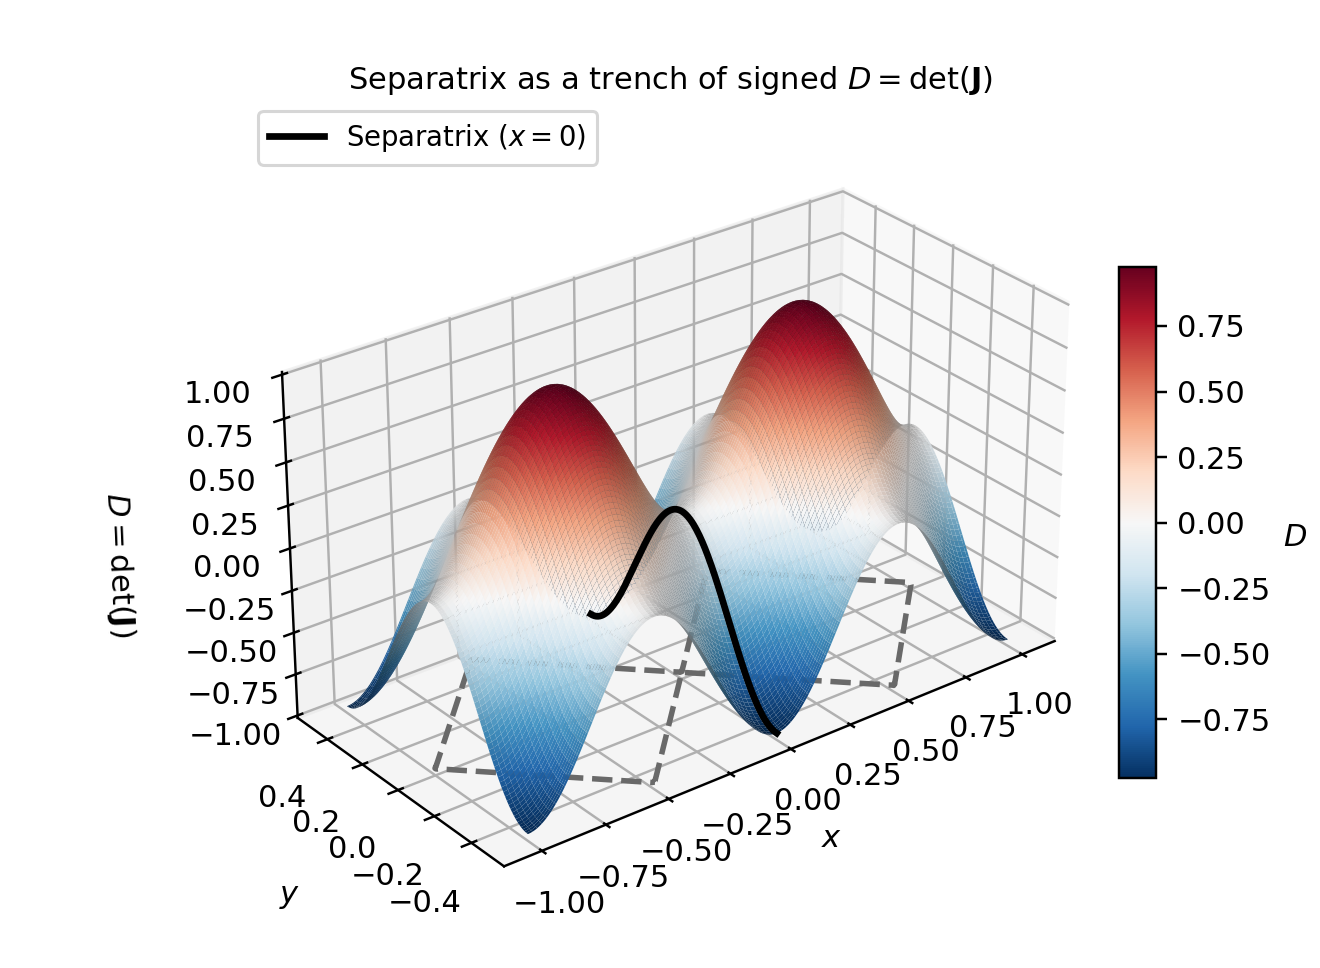
\includegraphics[width=0.40\textwidth]{figures/detJ_trench_cross_section.png}
    \caption{Signed $D$ as an elevation surface over the double gyre.
    The gyre cores rise as ridges ($D > 0$). The separatrix at $x = 0$
    (bold) is a trench of $D$, deepest at the saddles and rising to
    $D = 0$ at the origin.}
    \label{fig:trench_cross}
\end{figure}

This gives two surrogate models for the separatrix. Both have companion
features in the quadratic fit, making this a matter of navigating a
scalar field invariant.

\section{Adaptive Navigation Primitives}
\label{sec:controllers}

This section derives the two primitives. They share the estimation
step, the saturation idiom, and the control architecture, and differ in
which term of (\ref{eq:splitting}) each reads. The $D$ tracker reads
both, which buys it a noise margin; the $s_1$ tracker reads the strain
term alone, which buys it a frame-invariant target. That is the choice
the mission makes.

\subsection{Control Architecture}
\label{sec:arch}

Both primitives run inside the layered architecture established in
prior cluster space control studies \cite{8,31}, shown in
Fig.~\ref{fig:control_architecture} and described here from the bottom
up. The robot control layer consumes individual robot velocity
commands and emits actuation. The cluster space control layer consumes
a cluster-level command and emits those robot velocities through the
inverse kinematic Jacobian, and maps measured robot positions back
into cluster variables for feedback \cite{31,32}. The adaptive
navigation layer consumes the field samples returned by the six
robots, holds the estimator and
whichever primitive's control law is active, and emits a desired
centroid velocity $\dot{\mathbf{p}}_c$ together with the formation
setpoints. The state control layer sits on top, consuming the sensed
field quantities and the mission parameters and emitting the navigation
mode. It sequences acquisition, traversal, and terminal capture, applies
the hysteresis that keeps a noise-driven flicker from recycling a mode,
and responds to losing track of the feature of interest. Each layer
presents a fixed interface to the one above, so replacing the $D$
tracker with the $s_1$ tracker changes only the adaptive navigation
layer, the only layer that reads the field.

Cluster space control is an operational space control approach in
which the multirobot formation is represented as a virtualized full
degree-of-freedom articulating mechanism \cite{31}. The cluster-level
parameters are the cluster position, the cluster shape, and the
relative orientation of the robots with respect to the cluster. A
forward kinematic Jacobian maps robot-level velocities to cluster-level
velocities, and its inverse maps the cluster-level compensation
commands back to the individual robots.\footnote{Full dynamic control
is also possible via a Jacobian transpose transform; see \cite{31}.}
Lyapunov stability of the cluster space controller has been
characterized for arbitrary cluster space command trajectories, with
and without collision avoidance options \cite{32}. The cluster is the
pentagon-plus-center formation, its centroid
and heading following the command from above and each remaining cluster
variable regulated to its nominal shape value. Each robot is an
omnidirectional point mass.

\subsection{Robot Kinematics and Dynamics}
\label{sec:robot_model}

Each robot's velocity response is first order, $\dot{\mathbf{v}}_i =
(\mathbf{v}_i^{\text{des}} - \mathbf{v}_i)/\tau$, for commanded velocity
$\mathbf{v}_i^{\text{des}}$ and actuator time constant $\tau$.
Discretizing at control period $\Delta t$
gives the momentum model identified in \cite{8} on the Decabot, a
six-robot indoor omnidirectional testbed built for this work
\cite{33,34}:
$\mathbf{v}[k+1] = \alpha_{\text{mom}}\mathbf{v}[k] + (1 -
\alpha_{\text{mom}})\mathbf{v}^{\text{des}}[k]$,
where $\alpha_{\text{mom}} = e^{-\Delta t/\tau}$ gives $\tau = -\Delta
t/\ln\alpha_{\text{mom}} \approx 0.28$~s at $\Delta t = 0.1$~s,
consistent with the identified Decabot lag. Each robot also carries a
speed limit and a stiction floor.
The primitives saturate each command channel through
$c_{\max}\tanh(c/c_{\max})$, so the commanded centroid speed never
exceeds $\sqrt{2}\,k\,c_{\max}$. A fixed navigation gain $k$ amplifies
the primitive command so that steady commands clear the stiction
floor. All gains are dimensionless, the Newton and gradient terms each
carrying an implicit per-step time unit absorbed into $k$, which at the
ocean operating point is the $600$~s step of
Section~\ref{sec:ocean_sim}.
Parameters are fixed across all experiments unless noted:
double gyre, $c_{\max} = 0.04$, $k = 3.0$,
$v_{\text{max,robot}} = 0.3$, $v_{\text{stiction}} = 0.025$,
$\alpha_{\text{mom}} = 0.7$, $\rho = 0.075$, $\varepsilon_{\text{raw}} =
10^{-3}$, $\varepsilon_{\text{dim}} = 0.025$, $g_\perp = 1.0$,
$s_{\mathrm{trim}} = 0.05$, $g_{\text{capture}} = 0.15$, $r_{\text{band}}
= 0.05$; ocean, the same except $k = 1.8$, $v_{\text{stiction}} =
0.002$, $\alpha_{\text{mom}} = 0$, $\rho = 0.105$ ($1.4\times$, $5.4$~km),
and $s_{\mathrm{trim}} = 0.3$. The double-gyre column is
non-dimensional; Section~\ref{sec:ocean_sim} converts the ocean column
to physical units. The double-gyre
core wells have depth $s_1 = -\pi^2 A \approx -0.987$, well past
$-4s_{\mathrm{trim}}$ for the values above.

\begin{figure}[!t]
    \centering
    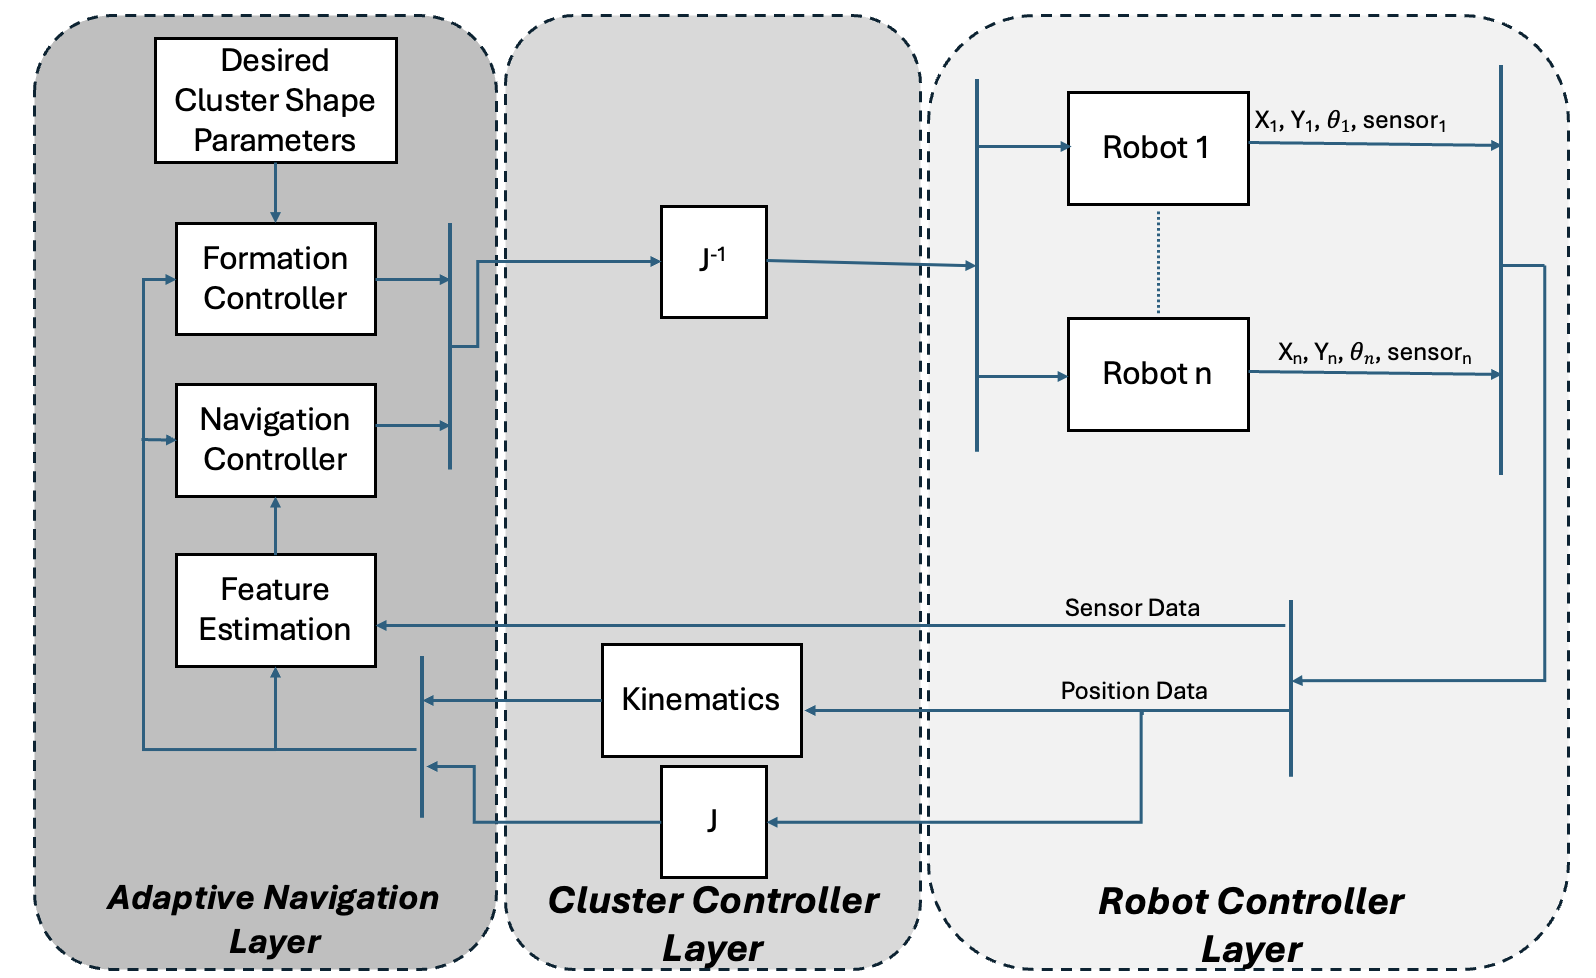
\includegraphics[width=0.40\textwidth]{figures/control_architecture.png}
    \caption{Hierarchical control architecture. Robot controller,
    cluster controller, and adaptive navigation layers, with the state
    control layer sequencing navigation modes above them.}
    \label{fig:control_architecture}
\end{figure}

\subsection{The $D$ Tracker}
\label{sec:sep_controller}

The $D$ tracker drives the cluster centroid onto the trench of $D$ and
then along it, following the separatrix through the crest that separates
one saddle from the next. Both motions are built from the local
quadratic surface the estimator returns.

The derivation works in the eigenbasis of the estimated Hessian. Let
$\hat{\mathbf{H}}_{D,0}\mathbf{w}_k = \lambda_k \mathbf{w}_k$ with
$\|\mathbf{w}_k\| = 1$ and $\lambda_1 \leq \lambda_2$. A trench of $D$
is convex across and concave along, so $\lambda_1 < 0 < \lambda_2$,
with $\mathbf{w}_2$ across the trench and $\mathbf{w}_1$ along it. The
sign of $\mathbf{w}_1$ is fixed so that $\hat{\mathbf{v}}_0^\top
\mathbf{w}_1 \geq 0$, which orients it downstream.

Because $\hat{D}$ is an exact quadratic surface, the Newton step
$-\hat{\mathbf{H}}_{D,0}^{-1}\hat{\mathbf{g}}_0$ reaches its stationary
point at once, but it cannot be issued as a velocity command.
It is a displacement, so commanding it as a velocity closes the whole
remaining distance in one unit of time and diverges as
$\hat{\mathbf{H}}_{D,0}$ approaches singularity, and the stationary
point it seeks is the crest, not a point on the separatrix. The first objection is met with the hyperbolic saturation
$\mathrm{sat}(c) = c_{\max}\tanh(c/c_{\max})$,
so that one parameter fixes both the transit speed and the width of the
terminal boundary layer. The second is met by treating the two
eigendirections separately, keeping the Newton component across the
trench and, along it, keeping only its magnitude and taking the
direction from the ambient flow.

The along-trench command changes character at the separatrix. Away from
it the along-trench gradient supplies a descent rate; on it that
gradient vanishes at the crest, so the flow supplies the speed instead.
The cluster is on the separatrix, $\mathbf{p}_c \in \mathcal{B}$, when
\begin{equation}
    |\hat{D}_0| < \varepsilon_{\mathrm{raw}}
    \quad\text{or}\quad
    \frac{|\hat{D}_0|}{\|\hat{\mathbf{H}}_{D,0}\|_F}
        < \varepsilon_{\dim},
\end{equation}
a raw threshold on the determinant or a curvature-normalized one, the
latter with units of length squared so the band scales with the
landscape, not with the absolute size of $D$. The along-trench
speed is then
\begin{equation}
    v_\parallel =
    \begin{cases}
        \hat{\mathbf{v}}_0^\top \mathbf{w}_1,
            & \mathbf{p}_c \in \mathcal{B}, \\[6pt]
        \dfrac{|\mathbf{w}_1^\top \hat{\mathbf{g}}_0|}{|\lambda_1|},
            & \text{otherwise},
    \end{cases}
    \label{eq:vpar}
\end{equation}
and the velocity command is
\begin{equation}
    \dot{\mathbf{p}}_c =
    \underbrace{\mathrm{sat}(v_\parallel)\,\mathbf{w}_1}_{\text{along the trench}}
    + \underbrace{\mathrm{sat}\!\left(-\frac{\mathbf{w}_2^\top
      \hat{\mathbf{g}}_0}{\lambda_2}\right)\mathbf{w}_2}_{\text{across the trench}},
    \label{eq:d_law}
\end{equation}
scaled by the navigation gain $k$ of Section~\ref{sec:robot_model}.

This control law decouples travel from trench holding through the
eigenbasis.
The across-trench term is the Newton component of the fitted quadratic,
normalized by the transverse curvature $\lambda_2$, and is the same
on and off the band, so the cluster is held to the trench at Newton rate
throughout. The along-trench term takes its direction from
$\mathbf{w}_1$, whose arbitrary eigensolver sign is
resolved against the measured flow to point downstream. Since
$v_\parallel \geq 0$ in both branches, the
along-trench motion never opposes the ambient flow. At a
crest the along-trench gradient vanishes while the separatrix continues
through, so the band test hands the speed to the measured flow.

When $\hat{\mathbf{H}}_{D,0}$ has eigenvalues of one sign the trench
frame is undefined. Off the band the law reverts to the signed Newton
step $\sum_k \mathrm{sat}(-\mathbf{w}_k^\top\hat{\mathbf{g}}_0/
\lambda_k)\mathbf{w}_k$, without a stability claim, and on the band to
the saturated flow alone. On the benchmark the fallback does not fire,
for a reason specific to that field (Section~\ref{sec:disc_limits}).

Convergence follows from the trench geometry. In arclength coordinates
$(\ell, n)$ along and across the trench, $D = h(\ell) +
\tfrac{1}{2}\kappa_\perp n^2$ with $\kappa_\perp = 2\pi^6 A^2 > 0$ along
a separatrix segment of the benchmark, so the transverse channel of the
$D$ law (\ref{eq:d_law}) reduces to $\dot{n} = -k\,\mathrm{sat}(a_\perp
n)$ with
$a_\perp = \kappa_\perp/\hat{\kappa}_\perp$, the ratio of the true
transverse curvature to the fitted one. Taking $V = \tfrac{1}{2}n^2$
gives $\dot{V} < 0$ for $n \neq 0$, so the cluster stays within the tube,
reaches the proportional region $|n| < c_{\max}/a_\perp$ in finite time,
and converges exponentially to the trench thereafter. Along the trench,
both branches of (\ref{eq:vpar}) keep $v_\parallel \geq 0$ and bounded
away from zero, so traversal cannot reverse and a segment
of length $L_\Gamma$ is crossed in time at most $L_\Gamma/(k\,m)$ for a
realized speed $m > 0$. Bounded estimation error $\delta$ leaves the
trench practically stable at $\limsup |n| \approx \delta/(k\,a_\perp)$,
where the zero-mean part of the error spreads the tracking error and the
truncation bias displaces it instead.

\subsection{The $s_1$ Tracker}

This primitive traverses the trench of $s_1$ using four quantities the
fit delivers, the eigenvalue $\hat{s}_1$, its gradient
$\nabla\hat{s}_1$, the strain eigenframe $(\mathbf{e}_1, \mathbf{e}_2)$,
and the deviatoric strain magnitude $r$, which measures how well resolved
that eigenframe is. The concavity of Section~\ref{sec:surrogates} rules
out a Newton snap on $s_1$, so both
channels of this primitive are built from the gradient.

The first step identifies the trench tangent. Naming an eigenvector
directly will not work, since $\mathbf{e}_1$ and $\mathbf{e}_2$ are
direction fields with no consistent sign, so the gradient is used. On the
trench the transverse derivative of $s_1$ vanishes by construction, so
away from a stationary point $\nabla\hat{s}_1$ points almost entirely
along the trench, and the tangent is whichever eigenvector the gradient
is less orthogonal to.
\begin{equation}
    \mathbf{t}_{\mathrm{raw}} =
    \arg\max_{\mathbf{e} \in \{\mathbf{e}_1, \mathbf{e}_2\}}
    \bigl\lvert \nabla\hat{s}_1^\top \mathbf{e} \bigr\rvert,
    \qquad
    \mathbf{t} = \mathrm{sgn}\bigl(\mathbf{t}_{\mathrm{ref}}^\top
    \mathbf{t}_{\mathrm{raw}}\bigr)\,\mathbf{t}_{\mathrm{raw}},
    \label{eq:tangent_select}
\end{equation}
where $\mathbf{t}_{\mathrm{ref}}$ is the previous step's tangent once one
exists, or the measured flow $\hat{\mathbf{v}}_0$ on the
first tracking step. The rule selects $\mathbf{e}_2$ on the attracting
half of the separatrix and $\mathbf{e}_1$ on the repelling half, swapping
automatically through the origin. Continuity fixes only the residual
sign, not the direction.

The primitive alternates between traversing and settling, selected by a
ride flag $\beta \in \{0,1\}$ that is one while traversing, with velocity
command
\begin{equation}
    \dot{\mathbf{p}}_c =
    \beta\,c_{\max}\tanh(1)\,\mathbf{t}
    - \mathrm{sat}\!\bigl(g_\perp\,\mathbf{P}\,\nabla\hat{s}_1\bigr),
    \qquad
    \mathbf{P} = \mathbf{I} - \beta\,\mathbf{t}\mathbf{t}^\top,
\end{equation}
where $\mathrm{sat}$ saturates a vector's magnitude and preserves its
direction, reducing to the scalar saturation on any multiple of a unit
vector.

This control law decouples descent from travel through the projector.
With $\beta = 1$, $\mathbf{P}$ removes the along-trench component of the
gradient, so the cluster descends only across the trench while riding
along it at cruise speed $c_{\max}\tanh(1)$. With $\beta = 0$ the
projector becomes the identity, the ride term drops out, and the same
expression is full gradient descent on $\hat{s}_1$, settling at a
local minimum. The gain $g_\perp$ is fixed and not
curvature-normalized, so the transverse channel contracts at gradient
rate.

Two situations clear the ride flag, the state layer's mode
transitions. Before the cluster reaches any structure, $\beta = 0$
and the descent term homes onto the trench from anywhere in the basin.
First contact latches $\beta$ to one, when $\hat{s}_1$
first falls below $-s_{\mathrm{trim}}$. The second is the
terminal behavior, holding the cluster at a two-dimensional
stationary point of $\hat{s}_1$ when
\begin{equation}
    r > r_{\mathrm{band}}, \qquad
    \lVert\nabla\hat{s}_1\rVert < g_{\mathrm{capture}}, \qquad
    \hat{s}_1 < -4 s_{\mathrm{trim}}.
    \label{eq:capture_test}
\end{equation}

A flow saddle is not merely a crossing of two transverse trenches. It is
a genuine two-dimensional minimum of $s_1$, and on the benchmark this
is closed form: (\ref{eq:s1_analytic_main}) gives
$s_1 \geq -\pi^2 A$ with equality exactly at integer $(x_f, y_f)$, a
strict nondegenerate minimum with curvature $\pi^4 A$ on both axes. The
full gradient therefore collapses there, while at an
ordinary trench point it remains large along the trench even
though it vanishes across it, so gradient magnitude alone distinguishes
the two. This matters because the ambient flow also stagnates at a
saddle, starving any flow-based tangent rule of a direction exactly
where the ride needs one.
The three tests in (\ref{eq:capture_test}) reject, in order, the
isotropic point, an ordinary trench point, and a shallow flat spot of
$\hat{s}_1$ away from real structure. The $-4s_{\mathrm{trim}}$ depth
threshold is a hysteresis ratio, not a physical relation. The
condition arms at four times the first-contact depth and releases when
$\hat{s}_1$ rises back above $-s_{\mathrm{trim}}$, so a noise-driven
flicker of the gradient test does not send the cluster back through the
tangent comparison at the well, while a genuine departure still does.

One guard falls outside the control law. If the eigenframe is
degenerate, $r < r_{\mathrm{band}}$, and no previous tangent has been
established, then neither (\ref{eq:tangent_select}) nor continuity
supplies a direction. The command then rides the measured flow,
$\mathbf{t} = \hat{\mathbf{v}}_0/\|\hat{\mathbf{v}}_0\|$, with the
projector set to the identity. Only the first tracking step can reach
this case, and it is the one place in the primitive where the ambient
flow enters the command.

The transverse argument is the same, with one difference that decides
where the law can be used. The projector $\mathbf{P}$ at $\beta = 1$
removes the along-trench gradient, leaving the same transverse dynamics
$\dot{n} = -k\,\mathrm{sat}(a_\perp n)$, but with no curvature to
normalize by, the rate is set by the field, $a_\perp = g_\perp
\kappa_\perp(\ell)$, and $\kappa_\perp = \pi^4 A|\cos \pi y_f|$ vanishes
at the isotropic point at $y = 0$. The restoring force
disappears there, but so does the transverse gradient, so nothing steers
the cluster off the structure and the ride carries it across a ball of
radius $\epsilon$ in time $2\epsilon/(k\,c_{\max}\tanh 1)$ while $|n|$
grows by at most $O(\epsilon)$, after which exponential convergence
resumes. Traversal is immediate, since the tangential channel is
$c_{\max}\tanh(1)\,\mathbf{t}$ at constant speed with direction seeded
once by the measured flow, though that direction is only guaranteed
under exact estimates, and Section~\ref{sec:disc_noise} reports the
inversions that follow when it is seeded from a noisy fit.

\section{Simulation Program and Results}

\subsection{Simulation Setup}

A Python simulation implementing the architecture of
Section~\ref{sec:arch} evaluates both primitives.
The double-gyre experiments use the steady field of
Section~\ref{sec:dg_example} ($A = 0.1$) on $[-1, 1] \times
[-0.5, 0.5]$. The integrator is explicit Euler at 10~Hz ($\Delta t =
0.1$~s), robot dynamics follow the first-order model, and the cluster
layer distributes the centroid command through the analytic $12 \times
12$ inverse Jacobian while driving the nine formation shape terms to
nominal proportionally (gain 1.0 on lengths, 0.1 on angles, fixed
throughout). All trials use the nominal
formation with ring radius $\rho = 0.075$; a trial varies only the
formation's initial heading, drawn uniformly from $[0, 2\pi)$ in the
Monte Carlo sweeps and zero in the noise-free demonstration runs. The
cluster's angular velocity command is zero throughout, so
heading is held fixed at its draw, and the reported
ring-phase-dependent quantities are with respect to it. Clean trials
run 400 to 600 steps and stop at domain exit or, for the $D$ tracker,
150 steps after first saddle contact. Noise-sweep trials run up to 500
steps and stop at task completion or domain exit. The
estimator-accuracy sweep holds the formation static and draws
independent noise per trial.

Four experiment families exercise the primitives: noise-free
double-gyre runs from six matched starts, Monte Carlo sweeps over a
two-dimensional noise grid, a rotating-observer trial, and runs on a
measured ocean record. Each is described with its results below.

\subsection{Ocean HFR Setup}
\label{sec:ocean_sim}

The ocean experiment uses hourly surface-current frames for the Santa
Barbara Channel from the HFRNet U.S.~West~Coast Radial-to-Total Vector
product \cite{35}, on the $2$~km grid. The record is the one
\cite{26} uses, the same network over the same 28-h window, 29 frames
from May 16, 2012 08:00 GMT to May 17, 2012 12:00 GMT, so these results
are interpretable against prior work on it; no controlled head-to-head
against \cite{26} was run, since initialization and advection differ.
Frames are interpolated linearly in time. World
coordinates on $[-0.65, 0.65]^2$ map affinely onto a region centered on
$(34.2^{\circ}\mathrm{N}, -120.4^{\circ}\mathrm{W})$ spanning
$\pm 0.300^{\circ}$ of latitude and $\pm 0.363^{\circ}$ of longitude. The
$168$-step trial spans the full record.

Physical numbers follow from one unit block, length $L_w = 51.4$~km on
both axes and time $6000$~s, with a control period $\Delta t = 0.1$
time units, so one step advances the field by $600$~s and the
$168$-step trial covers the record. The commanded-speed cap
$\sqrt{2}\,k\,c_{\max}$ is then $0.87$~m/s. Because the longitude
half-extent is $0.3^{\circ}/\cos(34.2^{\circ})$, both axes carry the
same physical scale and the world-to-physical map is a uniform
dilation, so each zero set, trench, and extremum of $D$ and of the
strain eigenframe is the physical one. The FTLE reference uses the same
constants, so the controller and evaluation frames agree by
construction. Those fields come from subwindows of this record at two
horizons: the 24-h field of Fig.~\ref{fig:ocean_ftle} integrates the
first 25 frames, and the four-anchor persistence check uses 12~h.

Each departure from the double-gyre operating point is a trade against a
named quantity. The pentagon is
enlarged to $\rho = 0.105$, $1.4\times$ the nominal radius and $5.4$~km
at this site, trading truncation bias for noise suppression so the
footprint spans about five cells of the $2$~km grid rather
than under four. At one control cycle per ten minutes any vessel time
constant is negligible, so $\alpha_{\text{mom}} = 0$, and the stiction
floor drops to $0.002$, having no vessel-scale analogue. The navigation gain $k = 1.8$ follows the ridge branch that
makes landfall on the middle island. No noise level is estimated
for this field. The exactly-determined six-robot fit leaves no residual
to estimate $\sigma_{uv}$ from, and quantifying the uncertainty in ocean
data and its effect on tracking is, as \cite{26} concludes for this same
record, a harder problem left outside its scope. The noise model here is
validated on the double gyre only.

\subsection{Estimator Accuracy}
\label{sec:results_est}

\begin{figure}[!t]
    \centering
    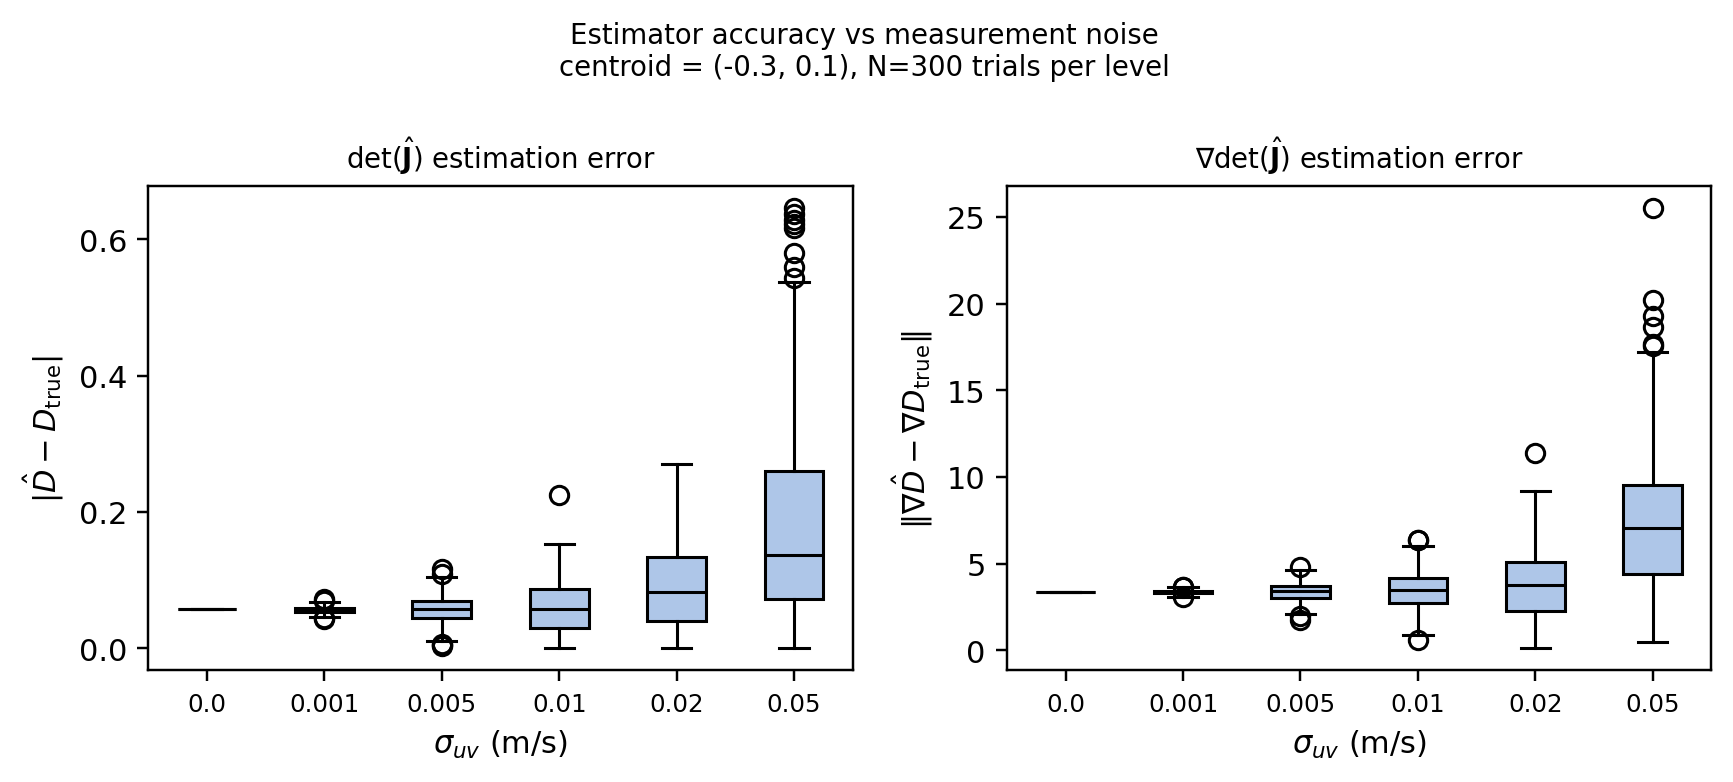
\includegraphics[width=0.9\columnwidth]{figures/estimator_accuracy_vs_noise.png}
    \caption{Estimator accuracy on the steady double gyre at the strain-region
    point $(-0.3, 0.1)$, $10^4$ noise draws per point. (a) Median relative error
    of $\hat{D}$, $\nabla\hat{D}$, and $\hat{\mathbf{H}}_D$ against measurement
    noise at $\rho = 0.075$; the dashed line marks error equal to signal, the
    dash-dotted line the $D$ tracker's 50\% traverse-success level. (b) Mean
    angle between the fitted and true principal eigenvector of
    $\hat{\mathbf{H}}_D$, against the $45^\circ$ of a uniformly random axis.
    The star is truncation acting alone.}
    \label{fig:est_accuracy}
\end{figure}

The estimator was characterized on the steady double gyre before any loop
was closed, over $10^4$ draws per condition at the strain-region point
$(-0.3, 0.1)$. The predictions of Section~\ref{sec:sensitivity} held.
Coefficient standard deviations matched the gain ladder
within 2.1\% and the reading error induced by
position noise matched (\ref{eq:sigma_eff}) within 1.6\%. The downward
bias of $\hat{s}_1$ matched prediction within 5\% in eighteen of
twenty-four conditions and within one standard error in all
twenty-four, the six wider cases sitting at $r/\sigma_r \geq
3$ where the predicted bias falls below the resolution of $10^4$
draws. The signed mean error of $\hat{D}$, $\nabla\hat{D}$, and
$\hat{\mathbf{H}}_D$ was zero to within 2.7\% of one standard deviation
across forty-eight conditions.
The correlation between the two component errors at one robot was $0.41$
under position noise against $0.44$ predicted, and zero under measurement
noise, which is the mechanism separating the channels.

In Fig.~\ref{fig:est_accuracy}(a), $\hat{D}$ stays informative to
$\sigma_{uv} \approx 0.07$ and $\nabla\hat{D}$ to $\approx 0.0075$, while
$\hat{\mathbf{H}}_D$ never falls below the error-equals-signal line at any
noise level, held there by $e_H$. In Fig.~\ref{fig:est_accuracy}(b),
truncation acting alone costs the $\hat{\mathbf{H}}_D$ eigendirections
$2.2^\circ$, while noise costs them $24^\circ$ by $\sigma_{uv} = 0.003$ and
$39^\circ$ at the closed-loop failure cliff, against $45^\circ$ for a
uniformly random axis.

The $s_1$ channel was checked at the nominal radius against its analytic
values, drawing $10^4$ realizations per condition at a fixed
strain-region point. The fitted shear strain at three test points is at
the $10^{-4}$ level (analytic value zero), and the fitted
$\hat{\mathbf{H}}_{s_1}$ eigenvalues are $[-0.011, 0.000]$ and smaller,
negative semidefinite as Section~\ref{sec:surrogates} requires. The
transverse component of the fitted gradient at $(0.03, 0.25)$, averaged
over ring phase, recovers a restoring slope of $6.83$ against the
analytic transverse curvature $6.888$, a full-sweep mean of $0.9$\%
truncation deficit. The spread across phases is the orientation
dependence, not scatter.
Rotating the ring through its $72^\circ$ period at the same point moves
the recovered slope between $4.0$ and $9.7$ about that mean of $6.83$,
and halving $\rho$ halves the spread, confirming the linear-in-radius
scaling. The mean tracks the analytic value, so the estimator is not
biased in the transverse channel. An individual formation orientation
is. At $\sigma_{uv} = 0.01$ the median direction error of
$\mathbf{e}_2$ is $4.5^\circ$, against $44^\circ$ for $\nabla\hat{s}_1$
and $41^\circ$ for the $\hat{\mathbf{H}}_D$ eigenvector ($2\times 10^4$
draws per level).

\subsection{Clean Runs}
\label{sec:disc_clean}

\begin{figure}[!t]
    \centering
    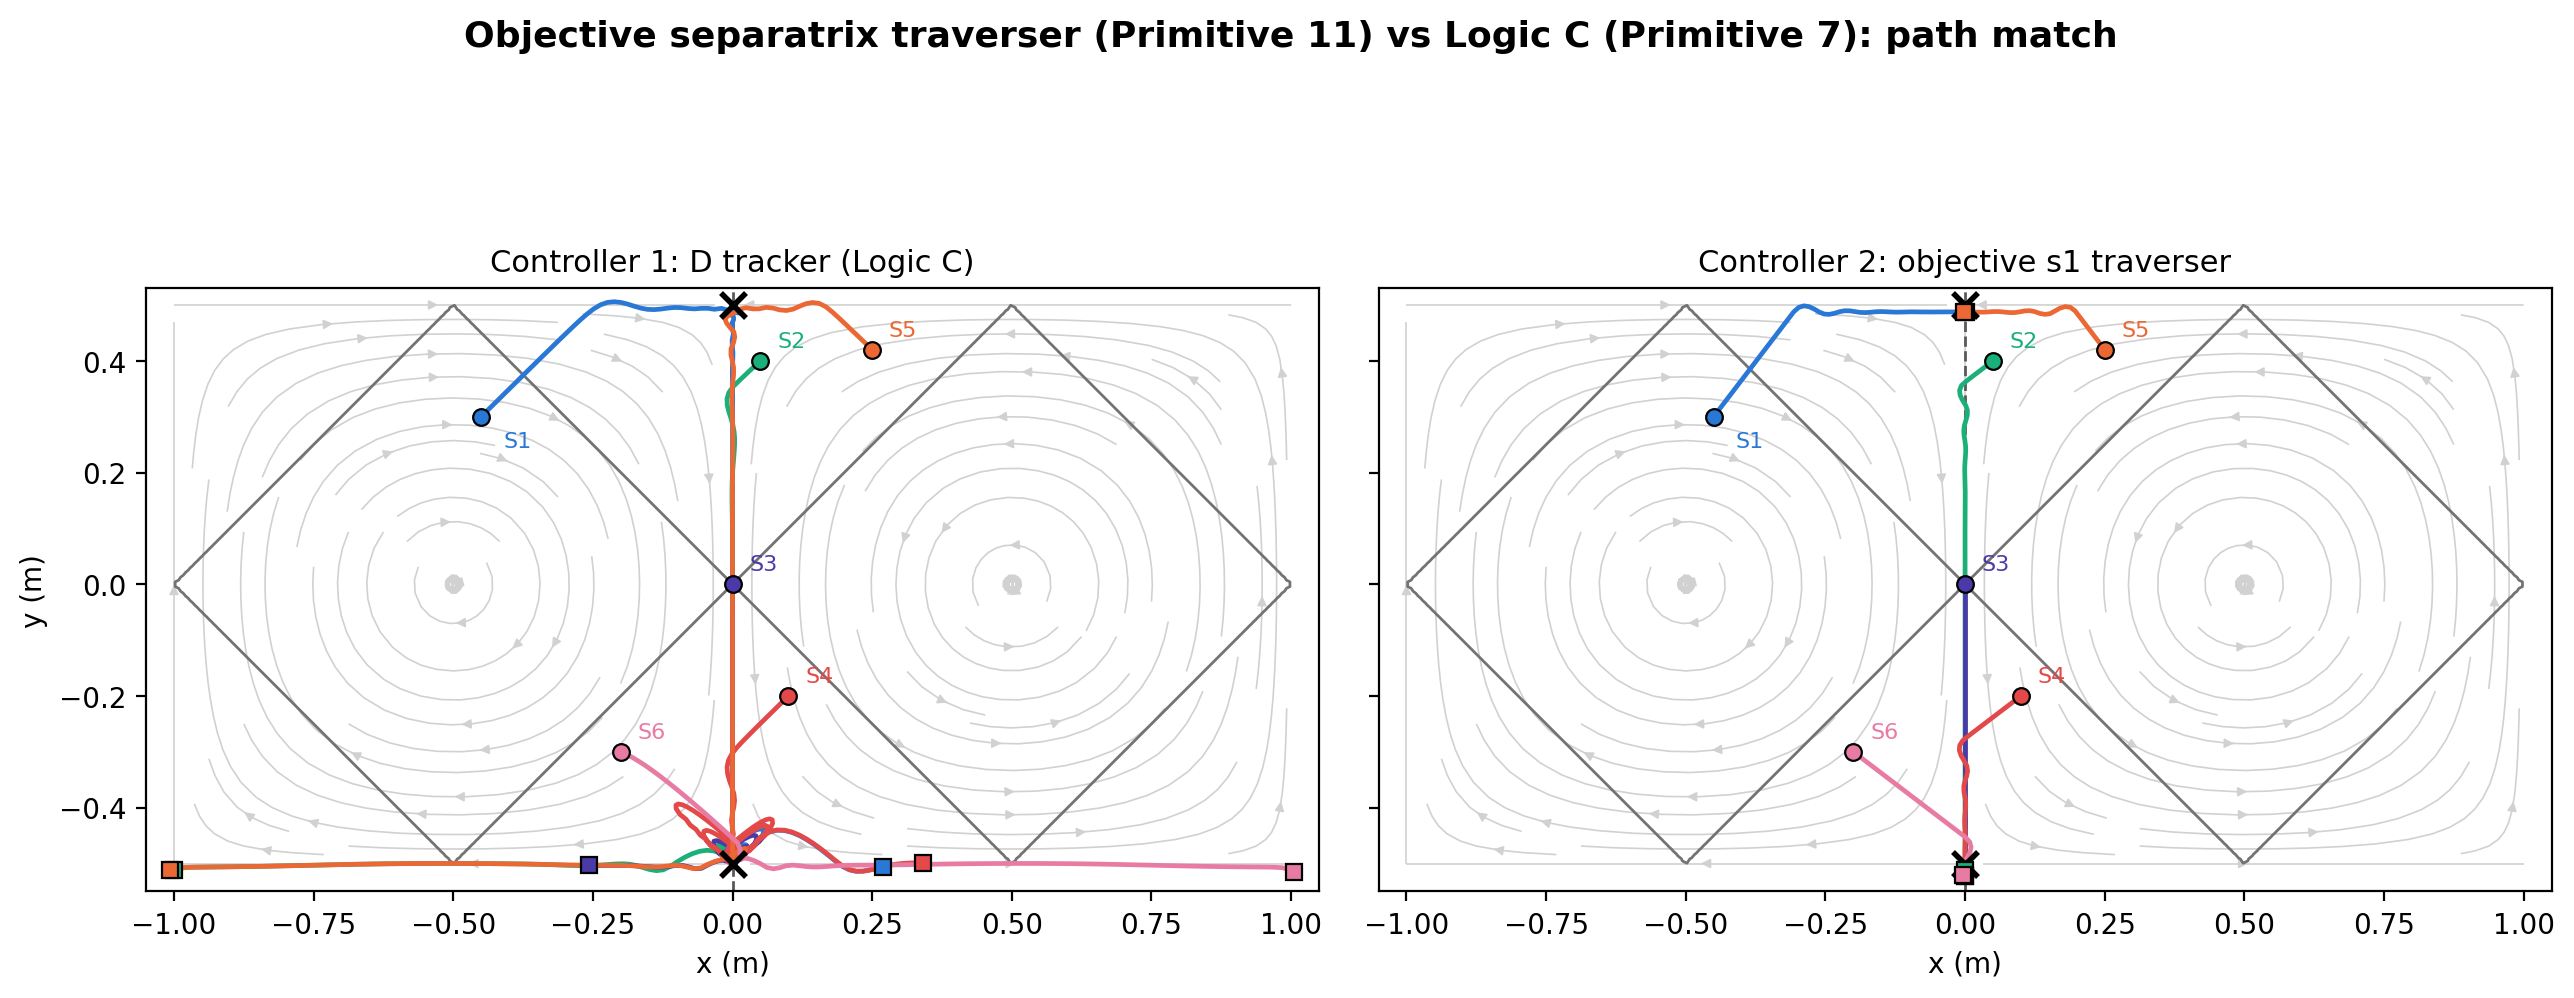
\includegraphics[width=0.44\textwidth]{figures/traverse_vs_logic_c.png}
    \caption{$s_1$ tracker versus $D$ tracker from six matched starts
    ($\bullet$), noise-free, overlaid on the double-gyre streamlines and
    Okubo-Weiss diamonds. Both traverse the same network through the
    isotropic point at the origin. The $s_1$ tracker captures at the
    saddle ($\times$) its tangent orientation resolves toward, while the
    $D$ tracker continues onto the crossing wall trench past each saddle
    it reaches, ending at the square markers.}
    \label{fig:traverse_vs_logic_c}
\end{figure}

These runs establish that both primitives work, and little more about
the comparison. The transverse derivatives of $D$ and $s_1$ vanish
together wherever the vorticity vanishes and the flow is
strain-dominated (\ref{eq:trench_coincide}), and the double gyre's
entire trench network is such a set, its vorticity identically
zero on the separatrix $x_f = 1$ and on all four walls, excepting only
the isotropic point at the origin. Whatever the two surrogates agree on
here, they agree on for a reason specific to this field.

Both were run noise-free from the same six starts
(Fig.~\ref{fig:traverse_vs_logic_c}), spanning both gyre halves, the
origin, and points off the structure entirely, between $0$ and $2.7\rho$
from the nearest trench segment ($\rho = 0.075$, the formation radius).
Both acquire the network from all six, in 6 to 35 steps for the $D$
tracker and 0 to 46 for the $s_1$ tracker, then ride the same segments
in the same direction and cross the isotropic point at the origin. A run
acquiring above the origin therefore rides an attracting OECS to that
point and continues onto a repelling one, on the same law and the same
scalar trench throughout. Neither needs dedicated machinery at the
crossing: the $s_1$ tracker rides through the origin on ordinary tangent
selection, and over a sweep of $r_{\text{band}}$ from 0.05 to 0 the
degenerate-frame guard never fires once.

The primitives part only at the terminal step
(Fig.~\ref{fig:traverse_vs_logic_c}), and the split is a fact about the
model class, not about tuning. The $s_1$ tracker
settles within 0.011 to 0.022 of a saddle in all six runs, at whichever
its initial tangent resolves toward, four at
$\mathbf{p}^*_1 = (0, -0.5)$ and two at $\mathbf{p}^*_2 = (0, 0.5)$. The
$D$ tracker passes within 0.02 of $\mathbf{p}^*_1$, then rides onto the
crossing wall trench and continues, because the capture test
$\lambda_1\lambda_2 \geq 0$ cannot fire. This
is neither a noise floor nor a tuning margin. By
Section~\ref{sec:sep_controller} the fitted $\hat{\mathbf{H}}_D$ is
traceless here, so its eigenvalues approximate
$\pm|\hat{H}_{xx}|$: at the well the estimated pair is
$[-0.51, 0.45]$ against a true $[18.3, 19.2]$, the induced trace being a
finite-radius truncation artifact. The same
limit binds in both directions, since $\hat{\mathbf{H}}_{s_1}$ is
negative semidefinite for every field and formation
(Section~\ref{sec:surrogates}), so neither surrogate admits a definiteness
certificate. The one terminal test a quadratic fit supports is a
vanishing gradient, and a flow saddle is a genuine two-dimensional
minimum of $s_1$, so that test is sufficient exactly where the $s_1$
tracker needs one and unavailable where the $D$ tracker would need one.
Traversal and capture are the same representability limit read twice.

The clean-field descent also fixes the reachable set, and it is not the
Okubo-Weiss partition. Over a 20\,000-cell start-position grid no run
settles at a gyre core, so descent of $\hat{D}$ leaves the
rotation-dominated interiors rather than stalling in them. The
reachable set is the watershed of that descent composited with the flow
direction on the acquired branch, whose arrival rate at
$\mathbf{p}^*_1$ is 47.4\% over that grid and 47.1\% over $n =
10{,}000$ random starts and headings. Prior AN primitives
\cite{3}, \cite{2} report local convergence without such an estimate.

A spot check on the time-varying double gyre \cite{26}, its separatrix
oscillating at $\varepsilon = 0.1$ and $\omega_{dg} =
2\pi/10$, runs the $D$ tracker down the oscillating trench at zero
noise. The trench swings $\pm 0.116$ in $x$
at a peak speed 62\% of the commanded cap, and the
primitive holds it with mean transverse offset 0.006 and maximum 0.015,
with no time-derivative term and no analytic guarantee for that case.

\subsection{Behavior Under Noise}
\label{sec:disc_noise}

\begin{figure}[!t]
    \centering
    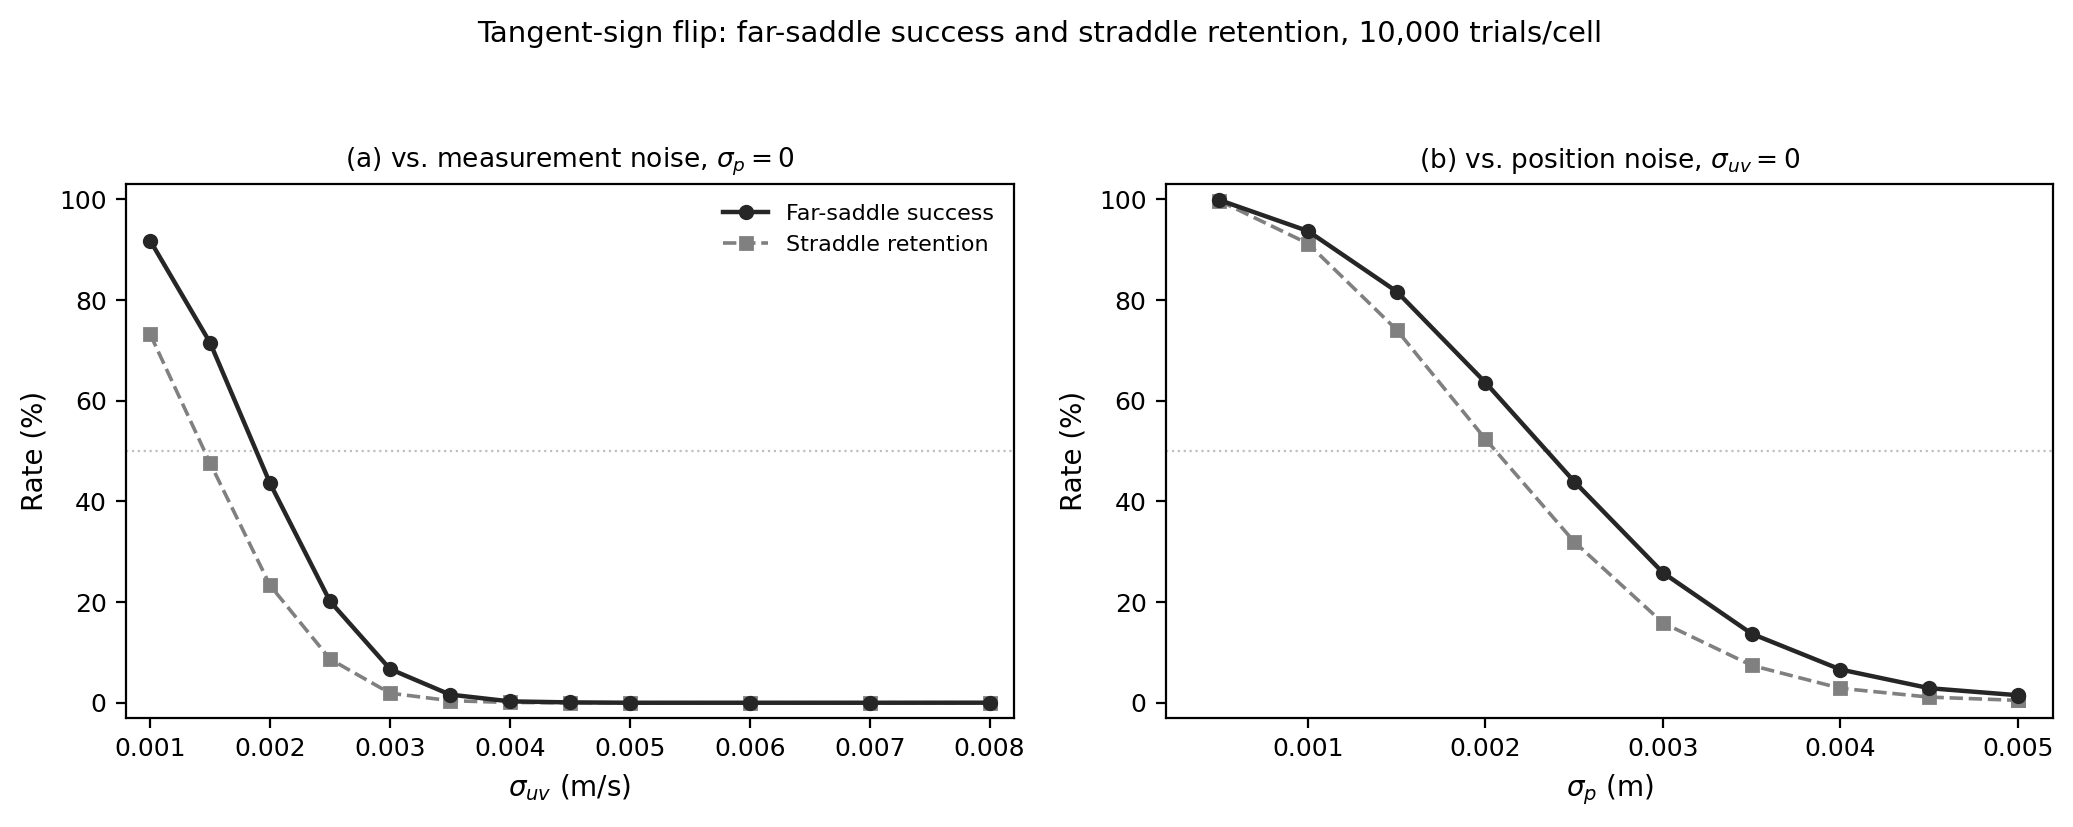
\includegraphics[width=0.9\columnwidth]{figures/flip_resolution.png}
    \caption{Resolving the tangent-sign flip. Far-saddle success and
    straddle retention (both conditioned on reaching $\mathbf{p}^*_1$),
    10\,000 trials/cell, at 0.0005 spacing on each axis. (a) Against
    $\sigma_{uv}$, $\sigma_p = 0$. (b) Against $\sigma_p$,
    $\sigma_{uv} = 0$. The transition is resolved and continuous on both
    axes; what is abrupt is the outcome it selects between.}
    \label{fig:flip_resolution}
\end{figure}

Both primitives sweep the same two-dimensional noise grid from one
straddling start, $(0, 0.35)$, at 10\,000 trials per cell, each from an
independent heading. Success is contact within 0.06 of the far
saddle $\mathbf{p}^*_1 = (0, -0.5)$, which a noise-free run from this
start reaches under either law, without formation collapse; each trial
also records straddle retention, the failure count of \cite{26}, and
tracking error. Holding one target fixed for both surrogates makes a
settle at the near saddle a directional failure rather than a loss of
the structure. Both start at 100\% with no noise, and noise then
separates them in favor of the $D$ tracker, whose 50\% crossing sits a
full grid step later, and the two fail differently.

For the $D$ tracker the cliff and an estimator threshold nearly
coincide. Success crosses 50\% at $\sigma_{uv} \approx 0.0079$, within
5\% of the $\sigma_{uv} \approx 0.0075$ at which $\nabla\hat{D}$ stops
being informative (Section~\ref{sec:results_est}). The gradient is not
the only input exhausted by then:
Fig.~\ref{fig:est_accuracy}(b) puts the curvature eigenframe $39^\circ$
from truth at the cliff against $45^\circ$ for a random axis, and both
terms of the $D$ law (\ref{eq:d_law}) are built on that frame. Neither
threshold is a property of the control law, so the estimator sets the
noise ceiling and the failure is a decay toward chance.

The $s_1$ tracker crosses 50\% between $\sigma_{uv} = 0.0015$ and 0.002
(Fig.~\ref{fig:flip_resolution}), and the cause has nothing to do with
estimator accuracy. On the separatrix $s_s \equiv 0$ and $\mu \equiv 0$,
so (\ref{eq:grad_s1}) collapses to $\nabla\hat{s}_1 = \pm(\hat{a}_5,
\hat{a}_4)$ and (\ref{eq:tangent_select}) reduces to the comparison
$|\hat{a}_5| > |\hat{a}_4|$, in which the true $a_5 = u_{xx}$ is
identically zero and $a_4$ collapses at both saddles, deciding at a
signal-to-noise ratio of $1.4$ at $\sigma_{uv} = 0.002$ against the
seed's $71$. Supplying one channel at a time confirms it: a clean flow
to the seed moves the correct-saddle rate at $\sigma_{uv} =
0.002$ from 44.6\% to 45.8\%, while a clean gradient and eigenframe to
the argmax moves it to 100\%. The cluster rides the separatrix
competently and settles in the wrong direction, a sign
inversion rather than a decay. Holding the tangent whenever the argmax
margin falls below the $\gamma_2\sigma_{\mathrm{eff}}/\rho^2$ the
gain ladder predicts for that comparison refuses the decision rather
than taking it at chance, on a derived threshold, and raises far-saddle
success from 44.6\% to 84.1\% at that level.

Two readings generalize past the sweep. The zero-noise tracking errors,
0.0075 for the $s_1$ tracker against 0.0016 for the $D$ tracker, have a
separate cause: both primitives park where their own transverse command
vanishes, which is where the \emph{fitted} trench lies and not the
field's, the gap being the orientation-dependent truncation bias. The
second is that robustness is set less
by the per-cycle accuracy of what a law reads than by how far a decision
is carried before it is checked against the world, the $D$ tracker
re-signing $\mathbf{w}_1$ against $\hat{\mathbf{v}}_0$ every cycle while
the $s_1$ tracker carries the sign in state through
$\mathbf{t}_{\text{ref}}$. That reliance is forced rather than chosen,
since objectivity rules out the fitted curvature
(Section~\ref{sec:surrogates}), the measured flow
(Appendix~\ref{app:equivariance}), and a world axis in turn, leaving the
law's own prior output. The sign recursion is the structural residue of
the objectivity commitment, not a weakness of this particular
law.

\subsection{Behavior Under a Rotating Observer}

\begin{figure}[!t]
    \centering
    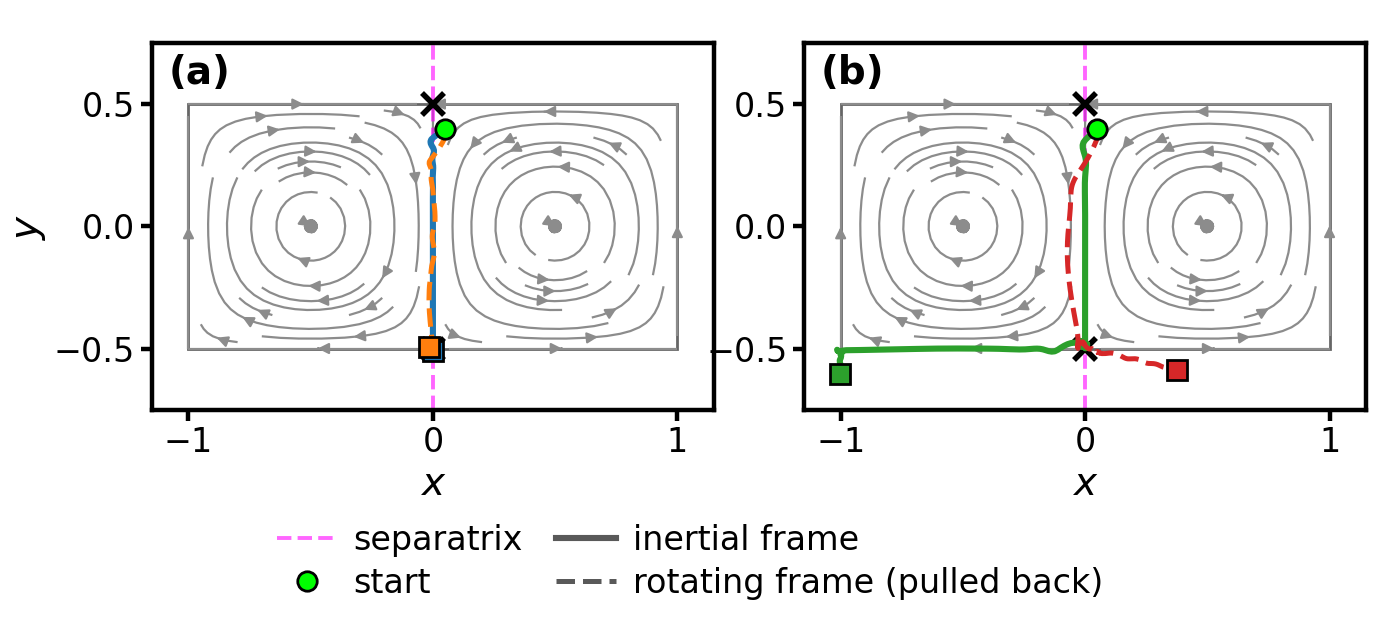
\includegraphics[width=\columnwidth]{figures/objectivity_traverser.png}
    \caption{Objectivity trial, both primitives started from
    $(0.05, 0.40)$ and run in the inertial frame (solid) and in a
    frame rotating at $\Omega = 0.2$ rad/s (dashed, pulled back to
    inertial coordinates). (a) the $s_1$ tracker's two runs coincide
    and capture at the same saddle (final gap
    0.025). (b) the $D$ tracker's rotating-frame run leaves the
    separatrix (final gap 1.219), the artifact predicted by
    (\ref{eq:D_not_objective}).}
    \label{fig:oecs_objectivity}
\end{figure}

Both primitives were run from $(0.05, 0.40)$, just inside the upper
saddle, on the same physical double gyre in two observer
frames: the inertial one and a frame rotating at $\Omega = 0.2$
rad/s, where the field is $\mathbf{v}'(\mathbf{p}', t) =
\mathbf{Q}\mathbf{v}(\mathbf{Q}^\top \mathbf{p}') + \Omega\,(-y',
x')^\top$. At a Rossby number $\mathrm{Ro} =
\lvert\omega\rvert_{\max}/2\Omega \approx 4.9$ the frame perturbs the
vorticity scale but not that of $D$, where
its effect is unbounded. The rate keeps the structure's apparent speed
at the tracked radius, $\Omega r \leq 0.10$, inside the command
authority $k\,c_{\max} = 0.12$, the condition the appendix requires.
Rotating-frame trajectories are pulled back to inertial coordinates and
compared with the inertial run of the same primitive.

The trial reverses the ranking
(Fig.~\ref{fig:oecs_objectivity}). The $s_1$ tracker's two runs are the
same material path, final gap 0.025 and mean gap 0.014, both capturing
at the same bottom saddle. The $D$ tracker's rotating-frame run does not
degrade. It leaves the structure, reaching a mean trench-network
distance ten times its inertial value of 0.005 and a final gap of 1.219
from the inertial run, ending in the gyre interior.

This is the observer term (\ref{eq:D_not_objective}) in closed loop. The
added solid-body vorticity moves the whole $D'$ landscape, and the same
rotation contaminates the flow measurement that the on-band branch of
the along-trench speed (\ref{eq:vpar}) reads, so both terms of the $D$
law (\ref{eq:d_law}) are steered by a frame artifact and not by the
field. No gain recovers this, because the artifact is in the surrogate,
and measured against $D$ itself it is unbounded exactly at the crest the
primitive must cross. The $s_1$ tracker inherits the protection of
Appendix~\ref{app:equivariance} instead, which exempts one instant and
holds only up to the frame-transport term, so the 0.025 gap is what it
predicts, not a violation of it.

The gain ladder places both surrogates on the same rung,
so the choice between them is not one of noise gain but of which
channels carry constants. Everything derived from $\hat{D}$ carries the
additive observer term of (\ref{eq:D_not_objective}), and
$\hat{\mathbf{H}}_D$ the unmodelled-derivative floor $e_H$ as well,
while $\hat{s}_1$ carries neither and is exposed instead at $1/r$, a
property of the strain field rather than of the sensing. Objectivity
costs the Newton normalization at the controller and a fitted trench
further from the true one at the estimator. The tangent the $s_1$
tracker rides comes from the
\emph{first-order} coefficients, one order better in noise gain than
the $\hat{\mathbf{H}}_D$ eigenvectors the $D$ tracker uses for the same
purpose, $4.5^\circ$ against $41^\circ$ at $\sigma_{uv} = 0.01$
(Section~\ref{sec:results_est}). That advantage belongs to the axis
itself; the argmax choosing which axis is tangent draws on the
second-order coefficients and is not better conditioned, which is where
Section~\ref{sec:disc_noise}'s failure sits.

\subsection{Behavior on a Measured Field}
\label{sec:disc_ocean}

\begin{figure}[!t]
    \centering
    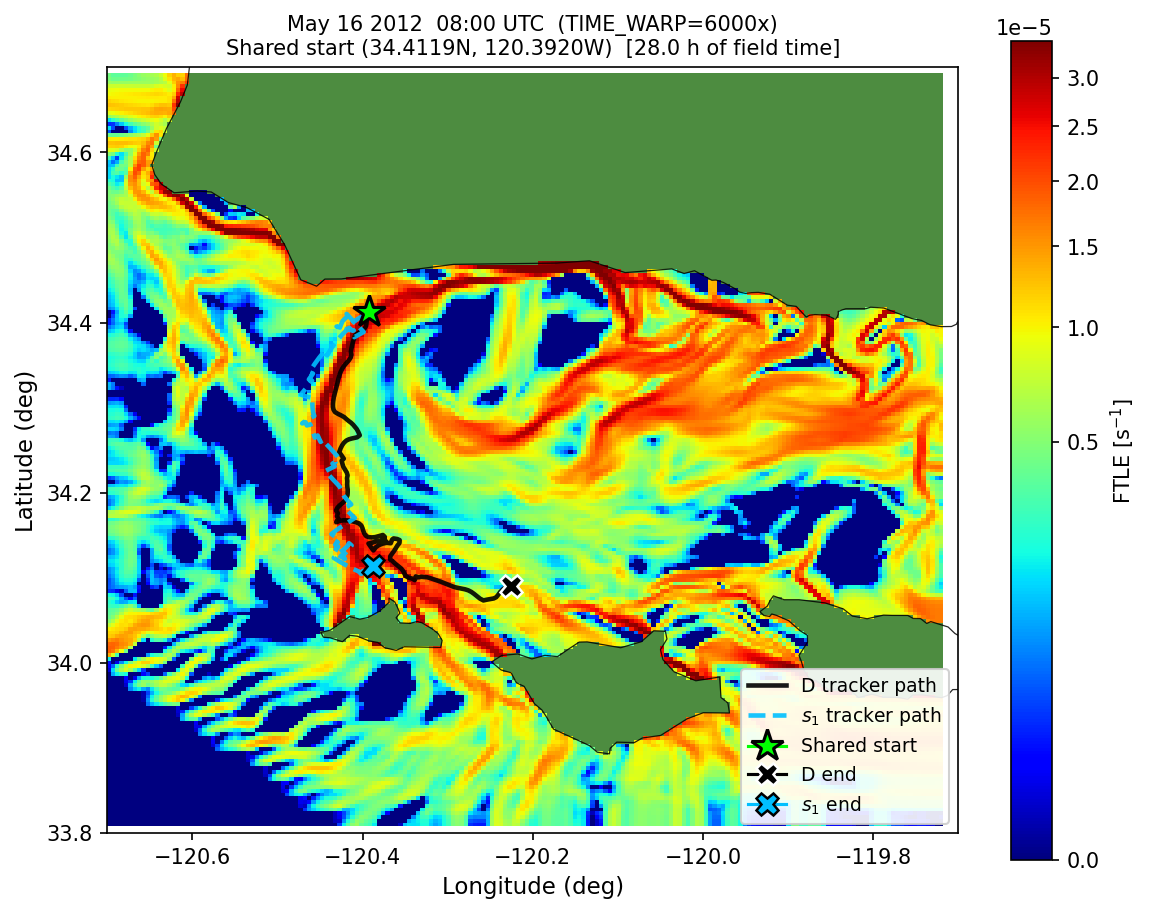
\includegraphics[width=0.38\textwidth]{figures/ocean_ftle_trajectory_overlay_2km.png}
    \caption{28-h $D$ and $s_1$ tracker paths, from a single shared
    start, over the 24-h forward FTLE field computed offline from the
    same 2~km data and anchored at the record start. Both follow the
    dominant ridge from the channel entrance to the bifurcation and
    separate only near landfall.}
    \label{fig:ocean_ftle}
\end{figure}

The ocean record removes the coincidence Section~\ref{sec:disc_clean} rests
on. A measured field has no reason to carry a vorticity-free trench
network, so nothing forces the two surrogates
onto a common curve. It also carries a nonzero horizontal
divergence, so $s_1 + s_2 = 2\mu$ no longer vanishes. That departure,
$2|\mu|/r$, has median
$0.8$--$1.1$ and 90th percentile $3.0$--$5.9$ along the two primitives'
paths, comparable to the deviatoric strain itself, so the
$s_2 = -s_1$ substitution of (\ref{eq:splitting}) is not tightly
bounded here and the splitting-identity reading of their agreement is
qualified accordingly. Both were run unmodified from a shared
start north of the channel entrance,
$(34.41^{\circ}\mathrm{N}, -120.39^{\circ}\mathrm{W})$, at the operating
point given above, and evaluated against the 24-h forward-time FTLE
field anchored at the record start. The $s_1$ tracker's depth condition latched at the first step and
stayed latched for the entire 168-step run, so the ride, not gradient
descent on an unlatched field, is what the record reports. Both spend
the record near the edge of their command authority rather than inside
it, the $D$ tracker reaching the $0.87$~m/s cap exactly against a
$0.71$~m/s mean, and the formation stays far from the conic degeneracy
throughout, at $\kappa(\boldsymbol{\Phi}) = 688$.
Over the 28~h trial both descend through
the channel entrance and track the same ridge through the bifurcation,
overlapping for nearly the entire record and separating
only at the end, where the $D$ tracker makes landfall on
the middle island while the $s_1$ tracker is still closing on
the same target.

What survives the loss of pointwise agreement is the corridor.
Fig.~\ref{fig:ocean_ftle} places both trials against the 24-h forward-time
FTLE field, computed offline in the style of
\cite{11}. Both follow the dominant ridge from the channel entrance to the
bifurcation closely: mean distance from the tracked path to the nearest
95th-percentile ridge point is 1.8~km for the $D$ tracker and 2.4~km for
the $s_1$ tracker (max 6.0 and 7.1~km), against the 2~km grid and the
5.4~km formation radius, with that ridge available to neither. Forward
FTLE recomputed at four anchor times (0, 5, 10, and 16~h, each
integrated 12~h forward) confirms that the dominant ridge
persists while the finer structure downstream evolves, and the $D$
tracker's outcome is insensitive to the start, 84 of 100
jittered starts on a $10 \times 10$ grid landing on the same
middle-island branch. Two primitives reading different halves of the
same splitting identity, from a shared start on a measured field, agree
on which corridor the transport skeleton occupies while disagreeing
about the trajectory inside it.

Instantaneous criteria of this kind are not in general reliable indicators
of the material transport skeleton \cite{16}. The double gyre is a
favorable special case, and this is a finding on one record, not a
guarantee that carries to arbitrary flows. The record is also
time-varying, each primitive seeing only the instantaneous samples at
its own formation position, with no analytic guarantee for that case.

The field is generic in a second way that matters for the $s_1$ tracker.
Its degeneracies are isolated and its cores move between frames, so the
trial exercises tangent selection where neither the eigenframe nor the
trench network is axis-aligned, which the double gyre cannot do. It
offers no genuine two-dimensional minimum of $s_1$ within reach of the
ride, so the capture test never engages and the same unmodified
primitive behaves as a traverser. Capture on the double gyre and
traverse on the ocean is a property of the field, not of a setting,
since the terminal test is unconditional by design.

\subsection{Limitations}
\label{sec:disc_limits}

The scope of the underlying framework should be stated plainly. Cluster
space control is centralized, requires global state, becomes intractable
for suitably large clusters, and is impractical without reliable
high-bandwidth communication among the robots \cite{31}. The claims here
are therefore made for small clusters operating in a limited workspace
with ample bandwidth, which is the regime the six-robot estimator
occupies by construction.

Within that regime, five limitations bear on the primitives. First, the
fit is ill-conditioned whenever the six sampling points drift toward a
common conic. No field tested here drives the formation toward one, so
the estimator is untested in the regime its own conditioning limit
describes, and the mitigation, monitoring
$\kappa(\boldsymbol{\Phi})$ with a shape-maintenance term, is not
implemented.
Second, noise can chatter the $D$ tracker across the band test
boundary, which costs speed alone, since both branches of the
along-trench speed share the same transverse dynamics. Third, the
strain eigenframe is fragile where $\mathbf{S}$ approaches isotropy,
the $1/r$ exposure of the estimator. Tangent selection is the defense once the ride is
underway, and the residual risk of a wrong branch at a crossing under
heavy noise is damped but not excluded by the capture test latch.

Fourth is the $s_1$ tracker's tangent rule. Its exposure
is the eigenvector comparison, so remedies aimed at
the seed do not reach it. The margin-hold rule of
Section~\ref{sec:disc_noise} recovers most of the loss without removing
the exposure, and two further changes remain unimplemented:
re-running the sign decision against the flow whenever the selected axis
changes, and, for a cluster with a trusted heading, resolving the sign
against a world axis every step.

Fifth, the $D$ tracker's traversal past a saddle is untested off the
benchmark. The true $\mathbf{H}_D$ is positive definite over the outer
half of each separatrix segment there, so the degenerate-frame fallback
should fire and does not: $u_{xx} = u_{yy}$
and $v_{xx} = v_{yy}$ on this field leave (\ref{eq:hess_det}) traceless,
its eigenvalues near $\pm|\hat{H}_{xx}|$. The fitted frame stays
indefinite by a symmetry of the field, not by a property of the
estimator.

No controlled head-to-head against the straddle family \cite{26,27,28} or
the onboard-FTLE strategy of \cite{30} was run: running those methods
from an off-structure start is outside their own stated problems, and
their robots are advected (eq.~1a in \cite{26}, eq.~5a in \cite{30})
while this paper's are not, so one simulator cannot host both unaltered. All
results are from simulation. The no-advection premise is exact for the
planned Decabot follow-on, where the field is encoded and read rather
than physically experienced \cite{34}, but on the ocean field it
is an extrapolation, untested against real advection.

\section{Conclusion}

This paper has presented two adaptive navigation primitives that
acquire, ride, and hold station on the instantaneous coherent
structures of a planar flow with a six-robot cluster, using only
synchronous local velocity measurements, with no map, no forecast, and
no assumption about the structure's identity. Both read the same
quadratic fit and present the same interface to the cluster space layer,
so switching surrogates costs one function call, not a
new estimator or a new controller.

The experiments give an operational selection rule. With a noisy sensor
the $D$ tracker holds a full grid step longer, its ceiling set by the
estimator rather than by its own law. Under a rotating observer the
ranking reverses: the $D$ tracker leaves the structure entirely, final
gap 1.219, while the $s_1$ tracker returns the same material curve in
both frames, final gap 0.025. On Santa Barbara Channel currents both
followed the same dominant transport corridor for 28 hours, within 1.8
and 2.4~km of an FTLE ridge neither could see, which is the bound this
sensing carries: instantaneous criteria resolve the corridor reliably
and the trajectory within it unreliably. The operator's choice
therefore depends on the observing platform, not on the flow. A cluster
that can certify its orientation should carry the $D$ tracker, which
tolerates a noisier sensor; a cluster that cannot should carry the
$s_1$ tracker, which alone returns the same material curve regardless
of frame.

The primitives are admittedly simple, reactive, and minimal in robot
count, consuming instantaneous information with no temporal filtering.
Without question, performance and robustness can be improved with
additional robots, filtering across control cycles, and more
sophisticated control laws. Even in their present form, however, they
demonstrate acquisition, traversal, terminal capture, and corridor
tracking on a measured record, which is the suite of behaviors a
structure-tracking mission requires.

Ongoing and future work is targeted at a) extending the stability
results to time-varying fields, b) online formation reshaping to
protect the conditioning of $\boldsymbol{\Phi}$ and to average out the
truncation bias that sets the zero-noise tracking error, c) verifying
and validating both primitives on the Decabot testbed and thereafter
with surface vessels, d) climbing the sensing ladder that relates a
feature class to the cluster that can resolve it, three robots for the
linear fit an isolated critical point needs \cite{8} and six for the
quadratic fit these structures need, with ten the next rung, whether
spent on a planar cubic or on a quadratic in three dimensions,
e) broadening the catalog of tracked features to transient attracting
profiles and eddy cores, and so on.

\appendices

\section{Frame Equivariance of the $s_1$ Tracker}
\label{app:equivariance}

Let an observer rotate as $\mathbf{p}_Q = \mathbf{Q}(t)\mathbf{p}$. The
strain tensor co-rotates and $s_1$ and $r$ stay invariant
(Section~\ref{sec:strain_field}), while the eigenframe and $\nabla s_1$
turn with the frame. Both tests the $s_1$ tracker performs, tangent
selection and the capture test, are scalar inequalities in those
invariants, so each returns the same verdict in every frame and the
command is equivariant, $\boldsymbol{\delta}_Q =
\mathbf{Q}\boldsymbol{\delta}$.

Equivariant commands do not by themselves give equivariant paths. A
rotating observer integrates $\dot{\mathbf{p}}_Q = k\boldsymbol{\delta}_Q$,
while the transported inertial path picks up the frame's transport
velocity, so the two separate at rate $\Omega\lVert\mathbf{p}_Q\rVert$.
That difference enters the transverse channel as a bounded disturbance,
so provided the frame turns slower than the cluster can correct,
$\Omega\lVert\mathbf{p}_Q\rVert < k\,c_{\max}$, the residue does not
accumulate and the tracker follows the same material structure in every
frame.

One step is exempt. The tangent is seeded once, at first contact, from
the measured flow, which is not objective, and that seed decides which
way the cluster rides. The frames agree while the transport
velocity perturbs the seed less than the flow supplies,
$\Omega\lVert\mathbf{p}_{\text{seed}}\rVert <
\lvert\hat{\mathbf{v}}_0^\top\mathbf{t}_{\text{raw}}\rvert$.
At the trial's start the right side is $0.096$ against
$0.081$, a margin of $1.19\times$ and a critical rate of
$\Omega \approx 0.238$ against the $\Omega = 0.2$ run. Should the
condition fail, the frames commit to opposite branches.

\begin{thebibliography}{99}
\bibitem{1} J. Cortés and M. Egerstedt, ``Coordinated control of multi-robot
systems: A survey,'' \textit{SICE Journal of Control, Measurement, and
System Integration}, vol. 10, no. 6, pp. 495--503, 2017.

\bibitem{2} C. A. Kitts, R. T. McDonald, and M. A. Neumann, ``Adaptive
navigation control primitives for multirobot clusters: Extrema finding,
contour following, ridge/trench following, and saddle point station keeping,''
\textit{IEEE Access}, vol. 6, pp. 17625--17642, 2018.

\bibitem{3} R. T. McDonald, C. A. Kitts, and M. A. Neumann, ``Navigation of
scalar fronts with multirobot clusters in simulation and experiment,''
\textit{IEEE Systems Journal}, vol. 14, no. 3, pp. 3755--3766, 2020.

\bibitem{4} L. Briñón-Arranz, A. Renzaglia, and L. Schenato, ``Multirobot
symmetric formations for gradient and Hessian estimation with application to
source seeking,'' \textit{IEEE Transactions on Robotics}, vol. 35, no. 3,
pp. 782--789, 2019.

\bibitem{5} P. Ögren, E. Fiorelli, and N. E. Leonard, ``Cooperative control
of mobile sensor networks: Adaptive gradient climbing in a distributed
environment,'' \textit{IEEE Transactions on Automatic Control}, vol. 49, no. 8,
pp. 1292--1302, 2004.

\bibitem{6} R. T. McDonald, C. A. Kitts, and M. A. Neumann, ``Experimental
implementation and verification of scalar field ridge, trench, and saddle
point maneuvers using multirobot adaptive navigation,'' \textit{IEEE Access},
vol. 7, pp. 62950--62961, 2019.

\bibitem{7} P. Keramea, K. Spanoudaki, G. Zodiatis, G. Gikas, and
G. Sylaios, ``Oil spill modeling: A critical review on current trends,
downscaling, and applications,'' \textit{J. Mar. Sci. Eng.}, vol. 9,
no. 2, art. 181, 2021.

\bibitem{8} C. Waight and C. A. Kitts, ``Adaptive navigation of multirobot
systems to critical points in 2D vector fields,'' submitted for publication.

\bibitem{9} G. Haller and G. Yuan, ``Lagrangian coherent structures and mixing
in two-dimensional turbulence,'' \textit{Physica D: Nonlinear Phenomena},
vol. 147, no. 3-4, pp. 352--370, 2000.

\bibitem{10} T. Peacock and G. Haller, ``Lagrangian coherent structures: The
hidden skeleton of fluid flows,'' \textit{Physics Today}, vol. 66, no. 2,
pp. 41--47, 2013.

\bibitem{11} S. C. Shadden, F. Lekien, and J. E. Marsden, ``Definition and
properties of Lagrangian coherent structures from finite-time Lyapunov
exponents in two-dimensional aperiodic flows,'' \textit{Physica D}, vol. 212,
no. 3-4, pp. 271--304, 2005.

\bibitem{12} M. Serra, P. Sathe, I. Rypina, A. Kirincich, S. D. Ross,
P. Lermusiaux, A. Allen, T. Peacock, and G. Haller, ``Search and rescue
at sea aided by hidden flow structures,'' \textit{Nature Communications},
vol. 11, no. 1, p. 2525, 2020.

\bibitem{13} J. Das, F. Py, T. Maughan, T. O'Reilly, M. Messié, J. Ryan,
G. S. Sukhatme, and K. Rajan, ``Coordinated sampling of dynamic oceanographic
features with underwater vehicles and drifters,'' \textit{The International
Journal of Robotics Research}, vol. 31, no. 5, pp. 626--646, 2012.

\bibitem{14} S. McCammon, G. Marcon dos Santos, M. Frantz, T. P. Welch,
G. Best, R. K. Shearman, J. D. Nash, J. A. Barth, J. A. Adams, and
G. A. Hollinger, ``Ocean front detection and tracking using a
team of heterogeneous marine vehicles,'' \textit{Journal of Field Robotics},
vol. 38, no. 6, pp. 854--881, 2021.

\bibitem{15} S. R. Ramp et al., ``Preparing to predict: the second autonomous
ocean sampling network (AOSN-II) experiment in the Monterey Bay,''
\textit{Deep Sea Research Part II: Topical Studies in Oceanography}, vol. 56,
no. 3-5, pp. 68--86, 2009.

\bibitem{16} G. Haller, ``Lagrangian coherent structures,'' \textit{Annual
Review of Fluid Mechanics}, vol. 47, pp. 137--162, 2015.

\bibitem{17} M. Serra and G. Haller, ``Objective Eulerian coherent
structures,'' \textit{Chaos: An Interdisciplinary Journal of Nonlinear
Science}, vol. 26, no. 5, p. 053110, 2016.

\bibitem{18} P. J. Nolan, M. Serra, and S. D. Ross, ``Finite-time Lyapunov
exponents in the instantaneous limit and material transport,''
\textit{Nonlinear Dynamics}, vol. 100, no. 4, pp. 3825--3852, 2020.

\bibitem{19} T. D. Harms, S. T. M. Dawson, and B. J. McKeon, ``Lagrangian
gradient regression for the detection of coherent structures from sparse
trajectory data,'' \textit{Royal Society Open Science}, vol. 11, no. 9,
p. 240586, 2024.

\bibitem{20} G. Haller, ``Dynamic rotation and stretch tensors from a
dynamic polar decomposition,'' \textit{Journal of the Mechanics and Physics
of Solids}, vol. 86, pp. 70--93, 2016.

\bibitem{21} A. Okubo, ``Horizontal dispersion of floatable particles in the
vicinity of velocity singularities such as convergences,'' \textit{Deep-Sea
Research}, vol. 17, no. 3, pp. 445--454, 1970.

\bibitem{22} J. Weiss, ``The dynamics of enstrophy transfer in two-dimensional
hydrodynamics,'' \textit{Physica D: Nonlinear Phenomena}, vol. 48, no. 2-3,
pp. 273--294, 1991.

\bibitem{23} J. C. R. Hunt, A. A. Wray, and P. Moin, ``Eddies, streams, and
convergence zones in turbulent flows,'' in \textit{Proc. Summer Program,
Center for Turbulence Research}, Rep. CTR-S88, pp. 193--208, 1988.

\bibitem{24} B.-L. Hua and P. Klein, ``An exact criterion for the stirring
properties of nearly two-dimensional turbulence,'' \textit{Physica D}, vol. 113,
no. 1, pp. 98--110, 1998.

\bibitem{25} C. Dong et al., ``Oceanic mesoscale eddies,'' \textit{Ocean-Land-
Atmosphere Research}, vol. 4, p. 0081, 2025.

\bibitem{26} M. Michini, M. A. Hsieh, E. Forgoston, and I. B. Schwartz,
``Robotic tracking of coherent structures in flows,'' \textit{IEEE Transactions
on Robotics}, vol. 30, no. 3, pp. 593--603, 2014.

\bibitem{27} M. Michini, H. Rastgoftar, M. A. Hsieh, and S. Jayasuriya,
``Distributed formation control for collaborative tracking of manifolds in
flows,'' in \textit{Proc. American Control Conference}, pp. 3874--3880, 2014.

\bibitem{28} M. Michini, M. A. Hsieh, E. Forgoston, and I. B. Schwartz,
``Experimental validation of robotic manifold tracking in gyre-like flows,''
in \textit{Proc. IEEE/RSJ International Conference on Intelligent Robots
and Systems (IROS)}, pp. 2306--2311, 2014.

\bibitem{29} G. Knizhnik, P. Li, X. Yu, and M. A. Hsieh, ``Flow-based control
of marine robots in gyre-like environments,'' in \textit{Proc. 2022 Int. Conf.
on Robotics and Automation (ICRA)}, pp. 3047--3053, 2022.

\bibitem{30} D. Kularatne and M. A. Hsieh, ``Tracking attracting manifolds in
flows,'' \textit{Autonomous Robots}, vol. 41, no. 8, pp. 1575--1588, 2017.

\bibitem{31} C. A. Kitts and I. Mas, ``Cluster space specification and control
of mobile multirobot systems,'' \textit{IEEE/ASME Transactions on Mechatronics},
vol. 14, no. 2, pp. 207--218, 2009.

\bibitem{32} T. Adamek, C. A. Kitts, and I. Mas, ``Gradient-based cluster space
navigation for autonomous surface vessels,'' \textit{IEEE/ASME Transactions on
Mechatronics}, vol. 20, no. 2, pp. 506--518, 2014.

\bibitem{33} S. Tomer et al., ``A low-cost indoor testbed for multirobot
adaptive navigation research,'' in \textit{Proc. IEEE Aerospace Conference},
pp. 1--12, 2018.

\bibitem{34} C. Waight and C. Kitts, ``A functional indoor testbed for
multirobot adaptive navigation in vector field environments,'' in
\textit{Proc. ASME Int. Design Engineering Technical Conf. and Computers
and Information in Engineering Conf.}, vol. 89251, 2025.

\bibitem{35} NOAA National Centers for Environmental Information,
``Near-real-time surface ocean velocities derived from HF-radar stations
[U.S. coastal waters],'' NCEI Accession
gov.noaa.nodc:IOOS-HFRadarRTVector.

\end{thebibliography}


\end{document}
